\chapter{Yield extraction}

\section{Fit description}
\label{sec:Lb_fit}

To extract the yields of the rare and resonant channels, an extended unbinned maximum likelihood fits are used.
%These are done simultaneously on the long and downstream samples.
The likelihood has the form:

\begin{equation}
\mathcal{L}=e^{-(N_\mathrm{S}+N_\mathrm{B}+N_{\mathrm{phsbg}})}\times\prod_{i=1}^{N}\left[
N_\mathrm{S}P_{\mathrm{S}}(m_i)+N_\mathrm{B}P_\mathrm{B}(m_i)+N_{\mathrm{phsbg}}P_{\mathrm{phsbg}}(m_i)\right]
\end{equation}
\noindent
where $N_\mathrm{S}$, $N_\mathrm{C}$ and $N_\mathrm{B}$ are number of signal, combinatorial and
\KS background events and $P_i(m_i)$ is the corresponding probability density function (PDF).
From now on when we refer to the invariant mass of the \Lb system we use the value obtained from
a kinematical fit of the full decay chain in which each particle is constrained to point to its
assigned origin vertex and the invariant mass of the $p\pi$ system is constrained to be equal to
the world average \Lz mass. In the resonant channel case a further constrain is used on the dimuon
mass to be equal to the known \jpsi mass. This method allows to improve the mass resolution giving
better defined peaks and therefore a more stable fit.

For the resonant channel the signal is described as a sum of two Crystal Ball functions (CB) with
common mean ($m_0$) and tail slope ($n$). A Crystal Ball function \cite{Skwarnicki:1986xj} is a probability
density function commonly used to model various processes involving energy loss. In particular it is used
to model the radiative tail which can be seen in many resonances' peaks. This function 
consists of a Gaussian core and a power-law tail, below a certain threshold. The function itself 
and its first derivative are both continuous and has form
%
\begin{equation}
C(x;\alpha,n,\bar{x},\sigma) = N \cdot
\begin{cases}
exp \left( -\frac{(x - \bar{x})^2}{2\sigma} \right)  & \mbox{   if   } \frac{(x - \bar{x})}{\sigma} > \alpha, \\
A\left( B - \frac{(x - \bar{x})}{\sigma} \right)^{-n} & \mbox{   if   } \frac{(x - \bar{x})}{\sigma} < \alpha,
\end{cases}
\end{equation}
%
where for normalisation and continuity
%
\begin{equation}
\label{CB}
\begin{array}{ll}
A = \left( \frac{c}{|\alpha|} \right))^n \cdot exp(- \frac{\alpha^2}{2}), \\
B = \frac{n}{|\alpha|} - |\alpha|.
\end{array}
\end{equation}
%
The full form of the PDF for the resonant channel is therefore:
%
\begin{equation}
P_\mathrm{S}(m;m_0,\alpha_1,\alpha_2,f,n) = f \text{CB}(m;m_0,\sigma_1,\alpha_1,n)+(1-f)\text{CB}(m;m_0,\sigma_2,\alpha_2,n),
\end{equation}
%
where $f$ is the relative fraction of candidates falling into the first CB function.

As a first step simulated $\Lb\to\Lz\mumu$ and \Lb\to\jpsi\Lz distributions are fitted using the signal PDF
separately for long and downstream candidates. Figure~\ref{fig:Lb_jpsiMCfit} shows simulated distributions
of resonant events with the fit function overlaid.

\begin{figure}
\centering
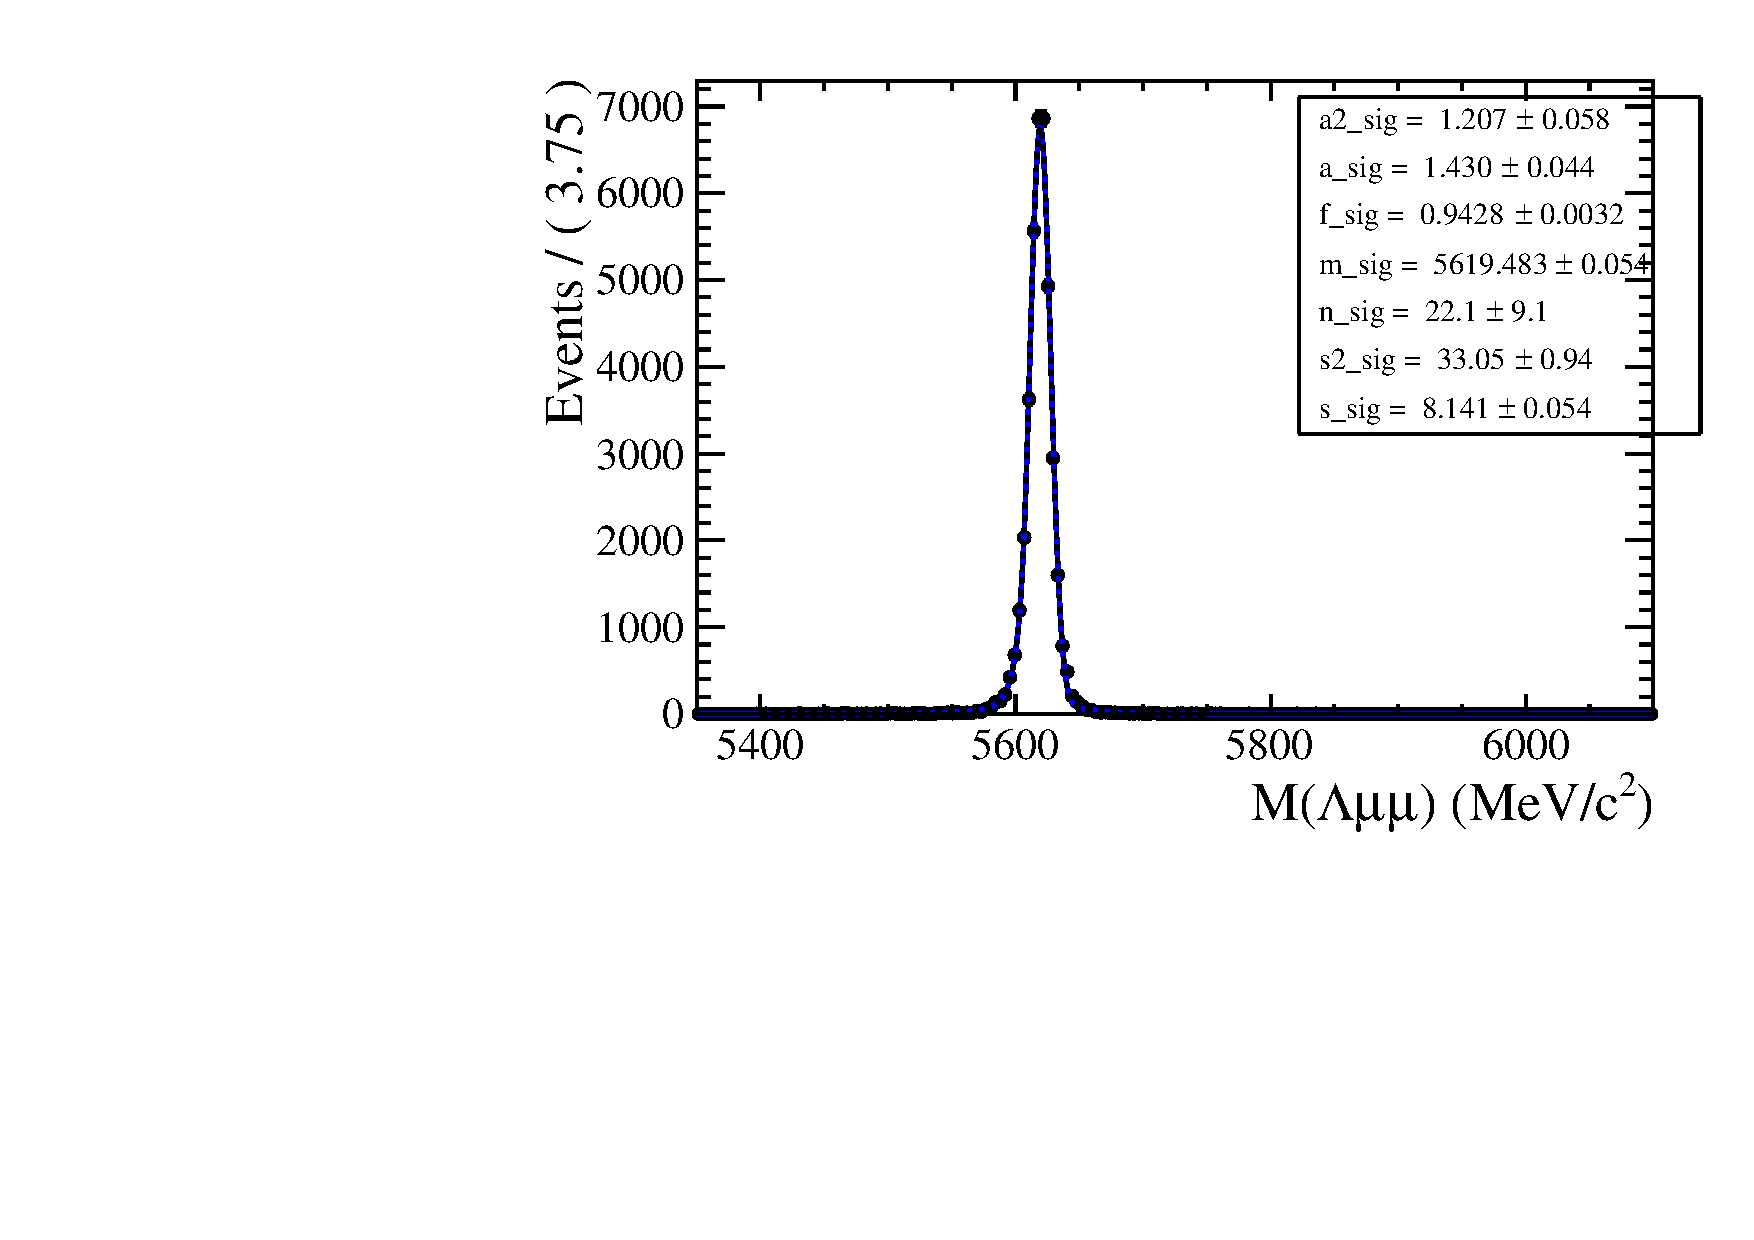
\includegraphics[width=0.45\textwidth]{Lmumu/figs/MassFits/fitLb2JpsiL_DD_MC.pdf}
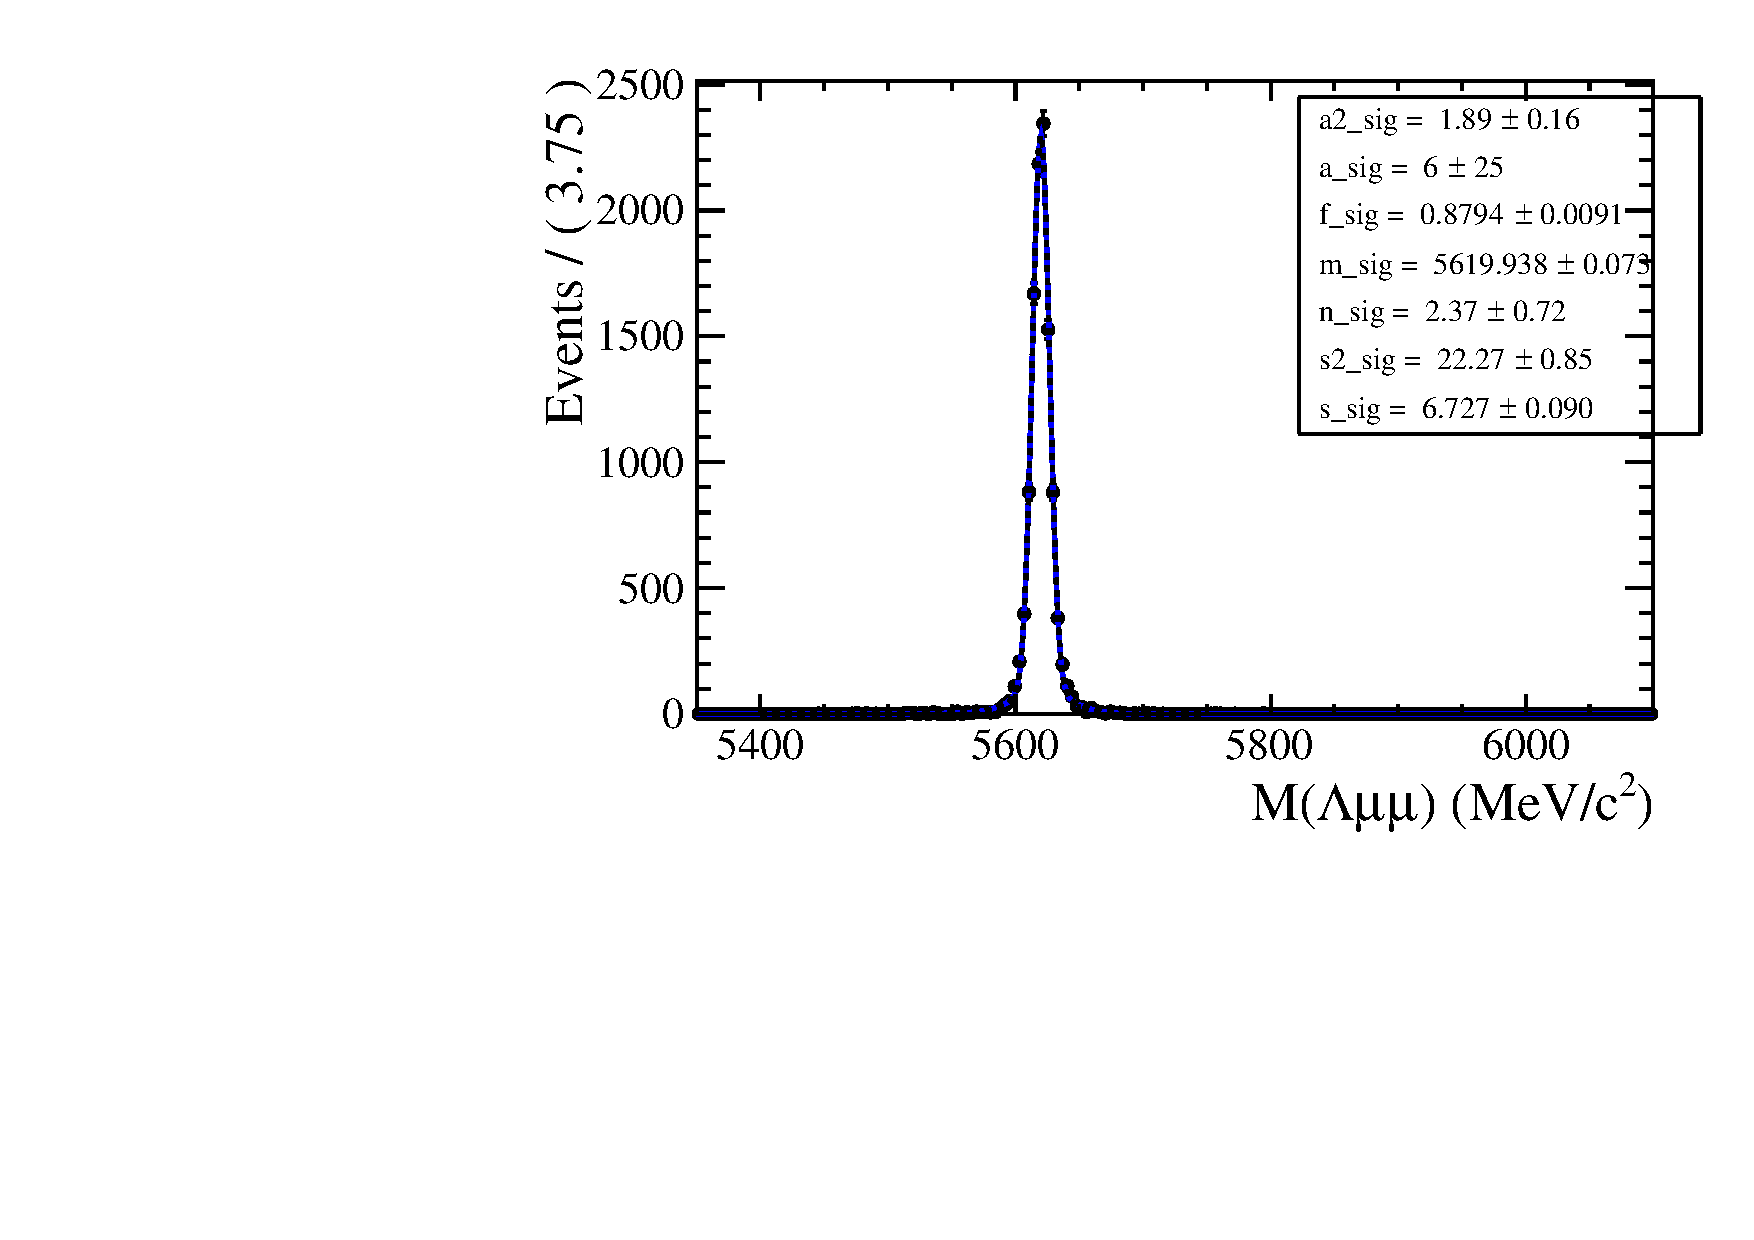
\includegraphics[width=0.45\textwidth]{Lmumu/figs/MassFits/fitLb2JpsiL_LL_MC.pdf}
\caption{Invariant mass distribution of $\Lb\ra\Lz\jpsi$ with fit and residuals for DD events (left) and LL events (right).
The histogram shows simulated data and the blue line is the signal fit function.}
\label{fig:Lb_jpsiMCfit}
\end{figure}

In a second step the fit to the resonant channel data sample is performed.
For the fit on data the tail slope parameter, ``$n$", which is higly correlated
with the $\alpha$s, is fixed it to the value found in the fit to simulated data.
In this fit two background components are modelled: the combinatorial background,
parameterized by an exponential and the background from $\Bz\ra\jpsi\KS$ decays.
The \KS background is described using the shape obtained using a $\Bz\ra\jpsi\KS$ simulated
sample and applying to it the full selection. The invariant distribution of these events
is fit with a Double Crystal Ball function, which is then used to model the \KS background
in the \Lb\to\jpsi\Lz fit. The fit to the simulated misreconstructed $\Bz\ra\jpsi\KS$ events
is reported in Fig.~\ref{fig:KSbkgFit}. When the \KS shape is introduced in the final fit all
parameters are fixed. This is particularly important when fitting long-long events, where the \KS
peak is less evident, which does not allow to constrain many parameters. On the other hand, in order
to take in account possible data-simulation differences, an horizontal shift is added and left
floating (by adding a constant to the central value, $m_0$ of the DCB).
In summary, the free parameters in the fit to the resonant \Lb\to\jpsi\Lz sample
are the yields of the signal and the combinatorial and \KS backgrounds, the slope
of the exponential and the horizontal shift of the \KS shape. Notice that all parameters
of the fit to the long and downstream samples are independent.

\begin{figure}
\centering
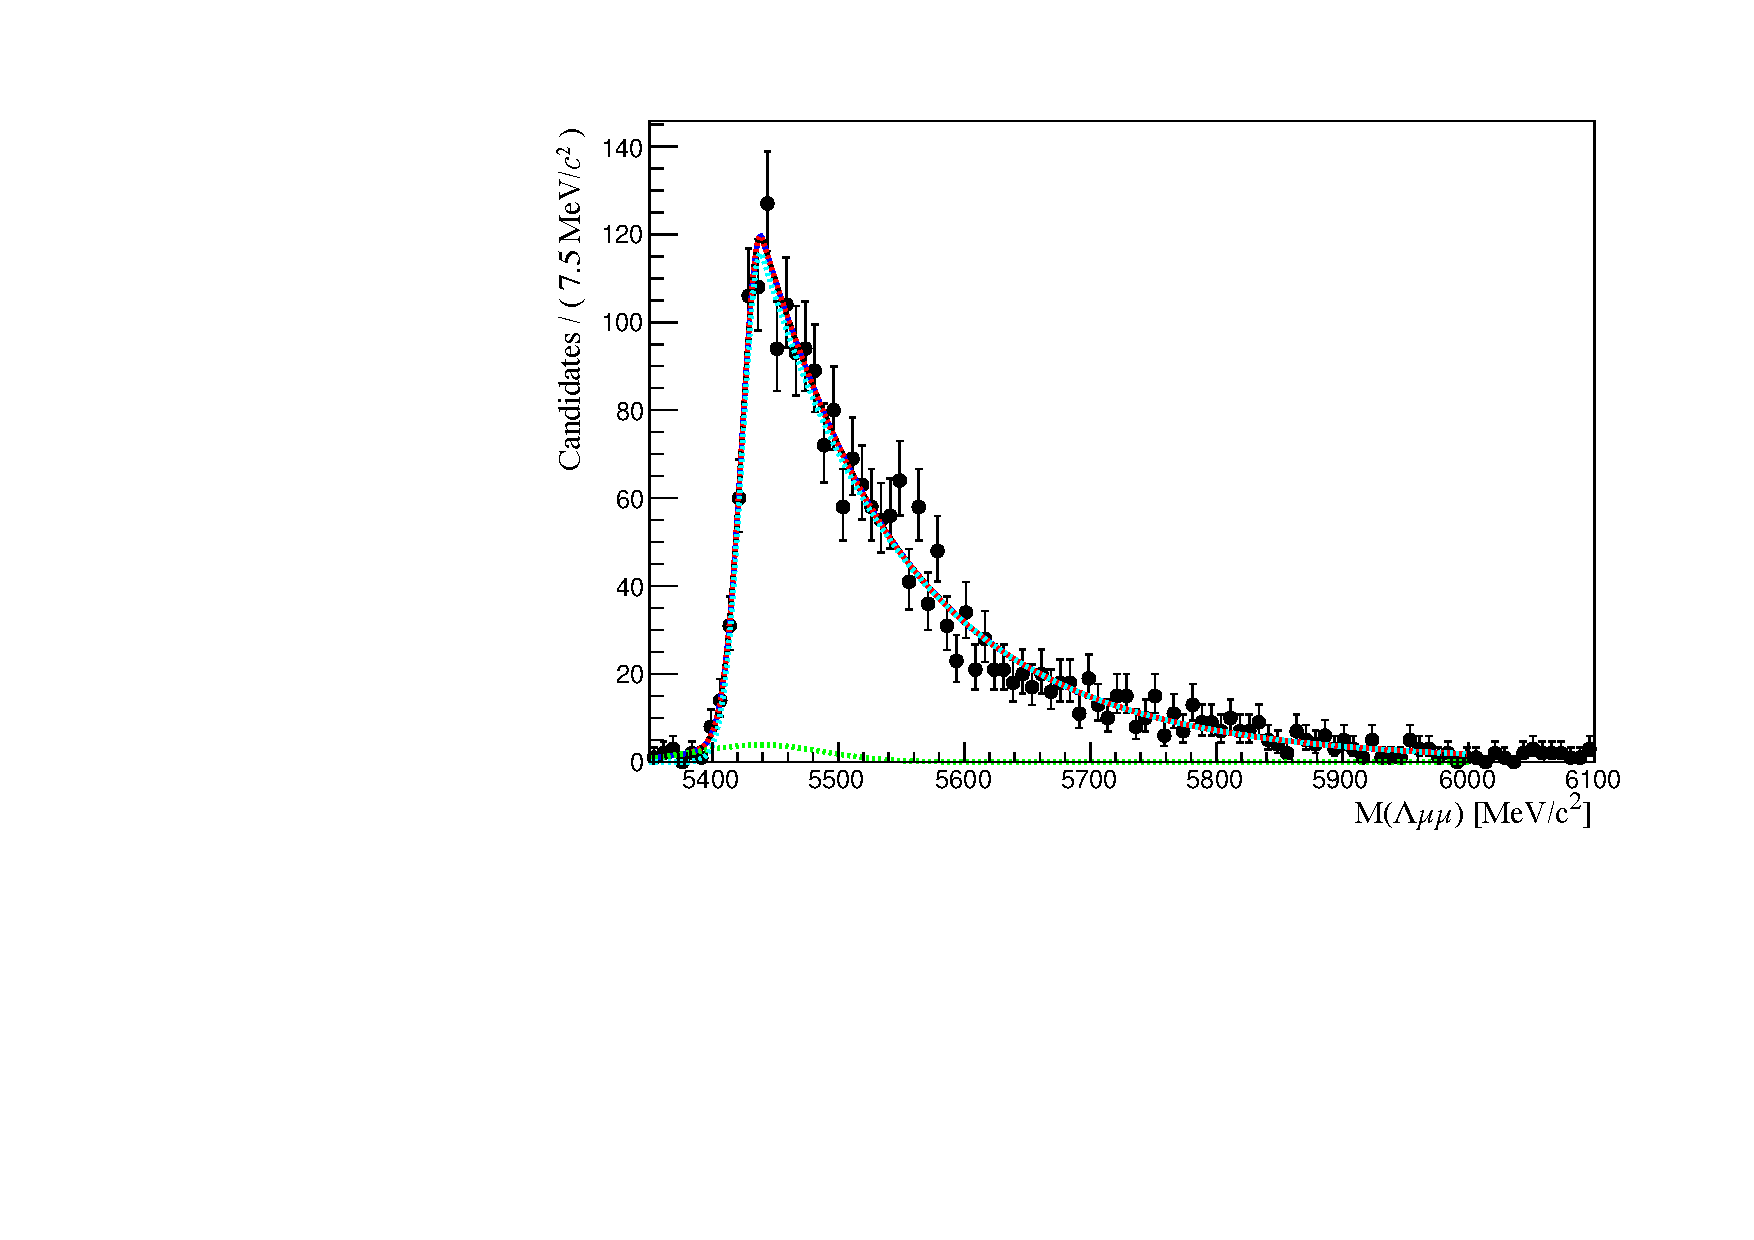
\includegraphics[width=0.45\textwidth]{Lmumu/figs/MassFits/fitKS_bkg.pdf}
\caption{Invariant mass distribution of simulated misreconstructed $\Bz\ra\jpsi\KS$ events after full selection fitted with Double Crystal Ball functions. }
\label{fig:KSbkgFit}
\end{figure}

Finally, the rare $\Lb\to\Lz\mumu$ sample is fit. In this case a simultaneous fit to the long
and downstream samples is performed to obtain a more stable convergence. 
In this fit the signal is modelled with the same shape used in the resonant case as there is no physical
reason why they should be different. This method is also useful to limit systematic uncertainties.
In fact the result will be given as a ratio between rare and resonant quantities.
However, the low statistics for the rare sample does not allow to constrain many parameters,
especially when dividing data in \qsq bins. Therefore, all parameters of the signal shape are fixed to
the ones derived from the fit on the normalisation channel. To account for possible differences, arising
for example from a different resolution in different \qsq regions, a scale factor is multiplied
to the width of the two gaussians cores at the signal DCB: $\sigma_1 \rightarrow c\cdot \sigma_1$
and $\sigma_2 \rightarrow c\cdot \sigma_2$, where the two scale factors are the same. This factors
are fixed in the fit on data by fitting a \Lz\mumu simulated sample in each \qsq bin and comparing
its widths with the ones found on the fit to the resonant simulated sample, namely
\begin{equation}
c = \sigma_{\mumu}^{MC} / \sigma_{jpsi}^{MC}.
\end{equation}
Values obtained are $\sim 1.9$ for downstream candidates and $\sim 2.3$ for long candidates,
corresponding to the fact that in the resonant case a further constrain on the dimuon mass
is used, which improves the resolution by a factor of 2. The of the scaling factor on \qsq is found to be small.
For fits on the DD and LL samples the parameters are always fixed to the corresponding \jpsi fit;
in this analysis parameters are never shared between DD and LL fits.

The background components modelled are also in this case
the combinatorial background, described with an exponential function. The slope of the background
is visibly different depending on the \qsq interval. This is partly due to the fact that,
at high \qsq, the combinatorial changes slope due to the kinematical limit at low masses.
The exponential slopes are therefore left floating independently in each \qsq bins 
and also independently of the resonant channel and for the in DD and LL samples.
The background component from \Bz\to\KS\mumu decays is modelled using the same shapes used
for the resonant channel. However, in this case the horizontal shift is fixed to what found
for the resonant channel. The expected amount of misreconstructed $\Bz\ra\KS\mumu$
events is small and does not allow to determine reliably the yield. Therefore, in the default
fit, this is fixed to the the yield of $\Bz\ra\jpsi\KS$ decays, rescaling it by the expected ratio
of branching fractions between the resonant and rare channels.
The \qsq distribution of $\Bz\ra\KS\mumu$ simulated events is then used to predict the yield as a function of \qsq.
In Tab.~\ref{tab:KSprediction} is reported the number of predicted $\Bz\ra\KS\mumu$ events in each \qsq bin 
obtained with the following formula:
\begin{equation}
N_{\KS\mumu}(\qsq) = N_{\jpsi\KS}\frac{B(\Bz\ra\KS\mumu)}{B(\Bz\ra\KS\jpsi)}\cdot \frac{1}{\epsilon_{rel}} \cdot B(\jpsi\ra\mumu) \frac{N(\qsq)_{MC}}{N^{tot}_{MC}} 
\end{equation}
where $N(\qsq)_{MC}$ is the number of simulated events in a \qsq bin after full selection and $N^{tot}_{MC}$ 
is the total number of simulated events. The \KS\mumu contribution is then completely taken out to study systematic
uncertainties as described in Sec.~\ref{sec:Lb_sys}
%Only for the 6-8 \gevgevcccc bin, a background component coming from the residual of the \jpsi radiative tail is
%added, modelled using a the shape obtained studying simulated events and smoothed using the \verb!RooKeysPdf! method of \verb!RooFit!.
%This is then removed from the final fit becuase it returns zero yield.

\begin{table}
\centering
\caption{Predicted numbers of $\Bz\ra\KS\mumu$ events in each considered \qsq interval.}
\begin{tabular}{lcc} \hline \hline
 \qsq interval [\gevgevcccc]  & Downstream & Long \\ \hline
0.1--2.0 & 0.9 & 0.1 \\
2.0--4.0 & 0.9 & 0.1 \\
4.0--6.0 & 0.8 & 0.1 \\
6.0--8.0 & 1.1 & 0.1 \\
11.0--12.5 & 1.9 & 0.2 \\
15.0--16.0 & 1.1 & 0.1 \\
16.0--18.0 & 2.0 & 0.2 \\
18.0--20.0 & 1.1 & 0.1 \\ \hline
1.1--6.0 & 2.1 & 0.1 \\
15.0--20.0 & 4.2 & 0.5 \\ \hline
\end{tabular}
\label{tab:KSprediction}
\end{table}

The fit on the rare sample is performed simultaneously on the LL and DD candidate categories.
Therefore the two separate yields are not separately floating but are but are parameterised
ad a function of the branching ratio with the following formula:

\begin{equation}
N(\Lz\mumu)_{k}  = \left[ \frac{\mathrm{d}\mathcal{B}(\Lz\mumu)/\mathrm{d}\qsq}{\mathcal{B}(\jpsi\Lz)} \right]  \cdot
N(\jpsi\Lz)_{k} \cdot \epsilon^{\mathrm{rel}}_{k} \cdot \frac {\Delta\qsq} { \mathcal{B}(\jpsi\to\mumu) },
\label{eq:relYield}
\end{equation}

where $k = $LL,DD, $\Delta\qsq$ is width of the \qsq bin and the only free paramater is the branching 
fraction ratio rare over \jpsi. For the \jpsi\to\mumu the value reported in the PDG book~\cite{PDG2014}, 
$\mathcal{B}(\jpsi\to\mumu) = (5.93 \pm 0.06)\cdot 10^{-2}$. In this formula the efficiencies and the normalisation 
yield appear as constants. These constants are then varied in order to obtain systemaitcs on the final result 
as described in Sec.~\ref{sec:Lb_sys}.


\section{Fit results}



\begin{figure}
\centering
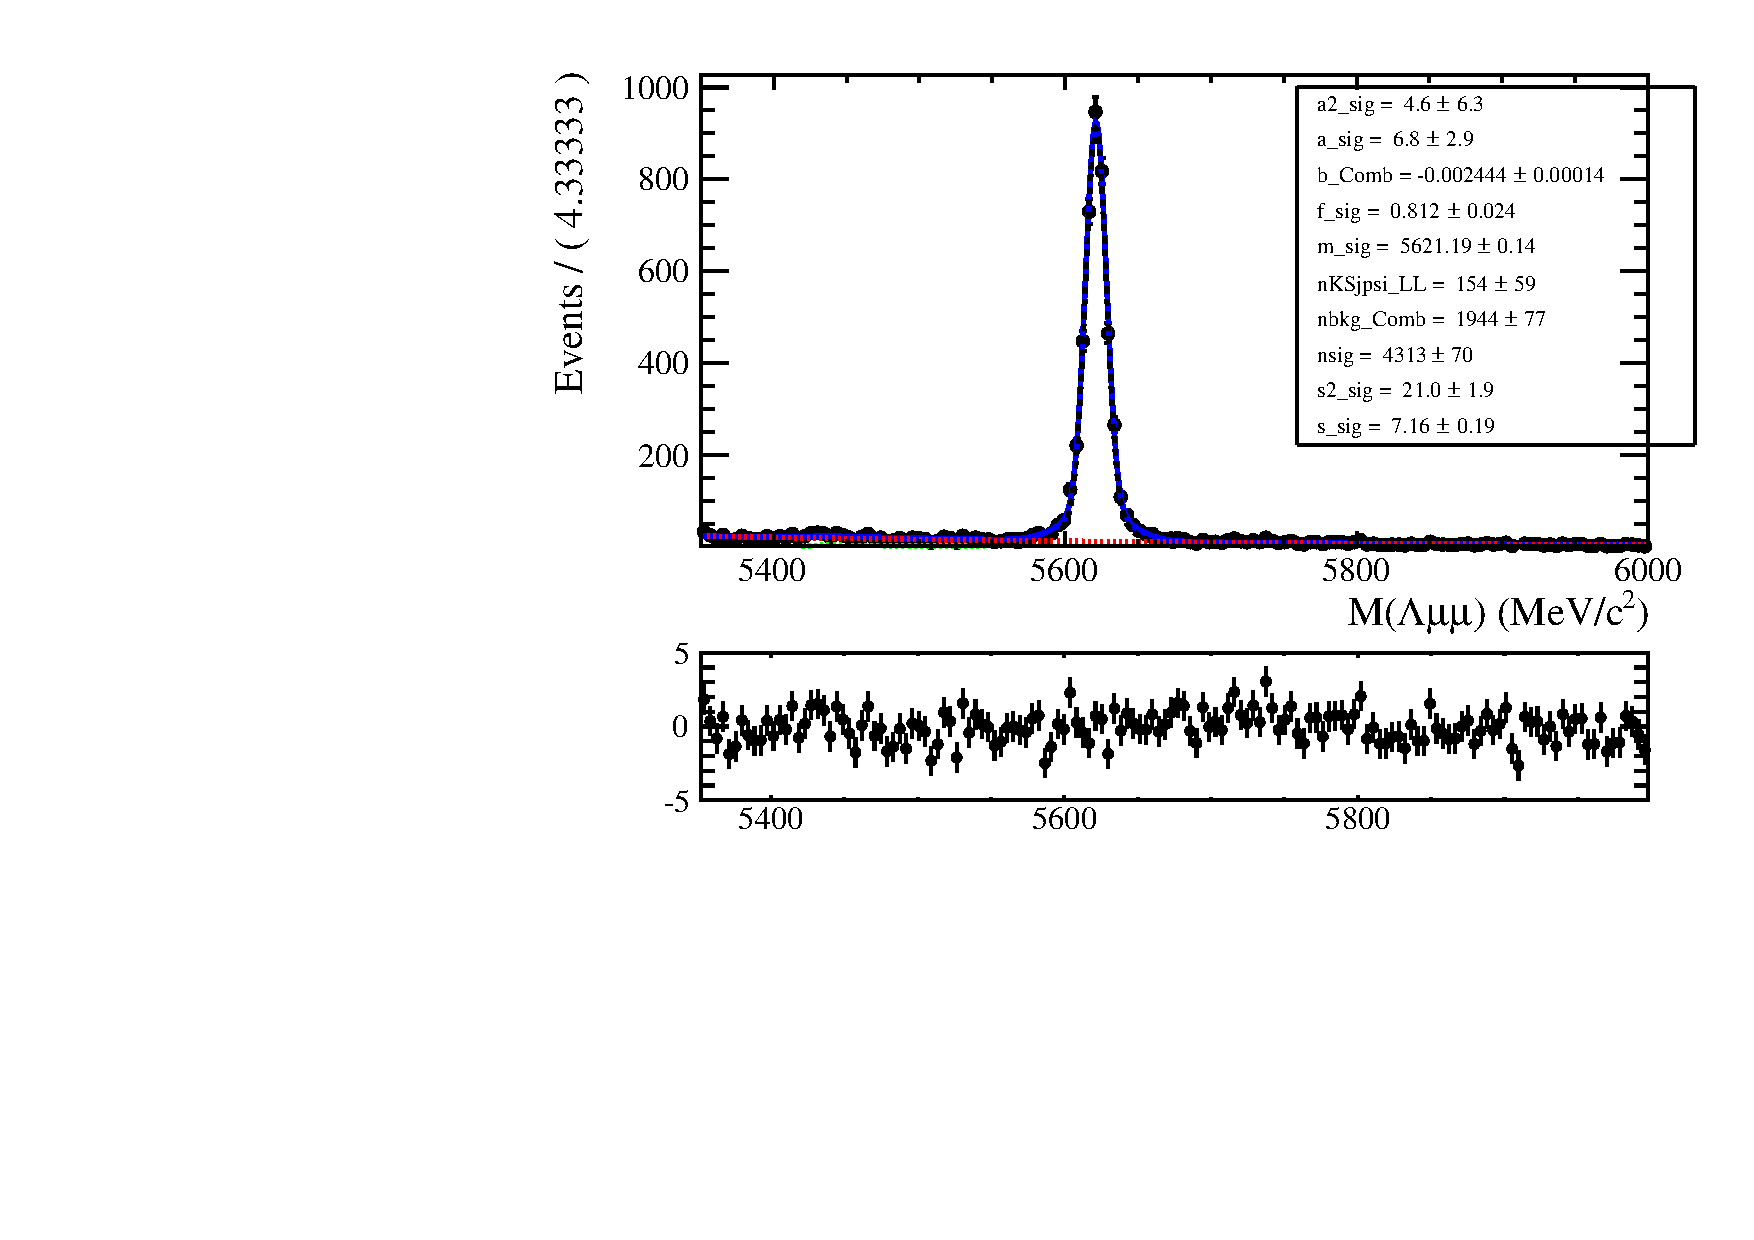
\includegraphics[width=0.45\textwidth]{Lmumu/figs/MassFits/Lb2JpsiL_LL_data_fitAndRes.pdf}
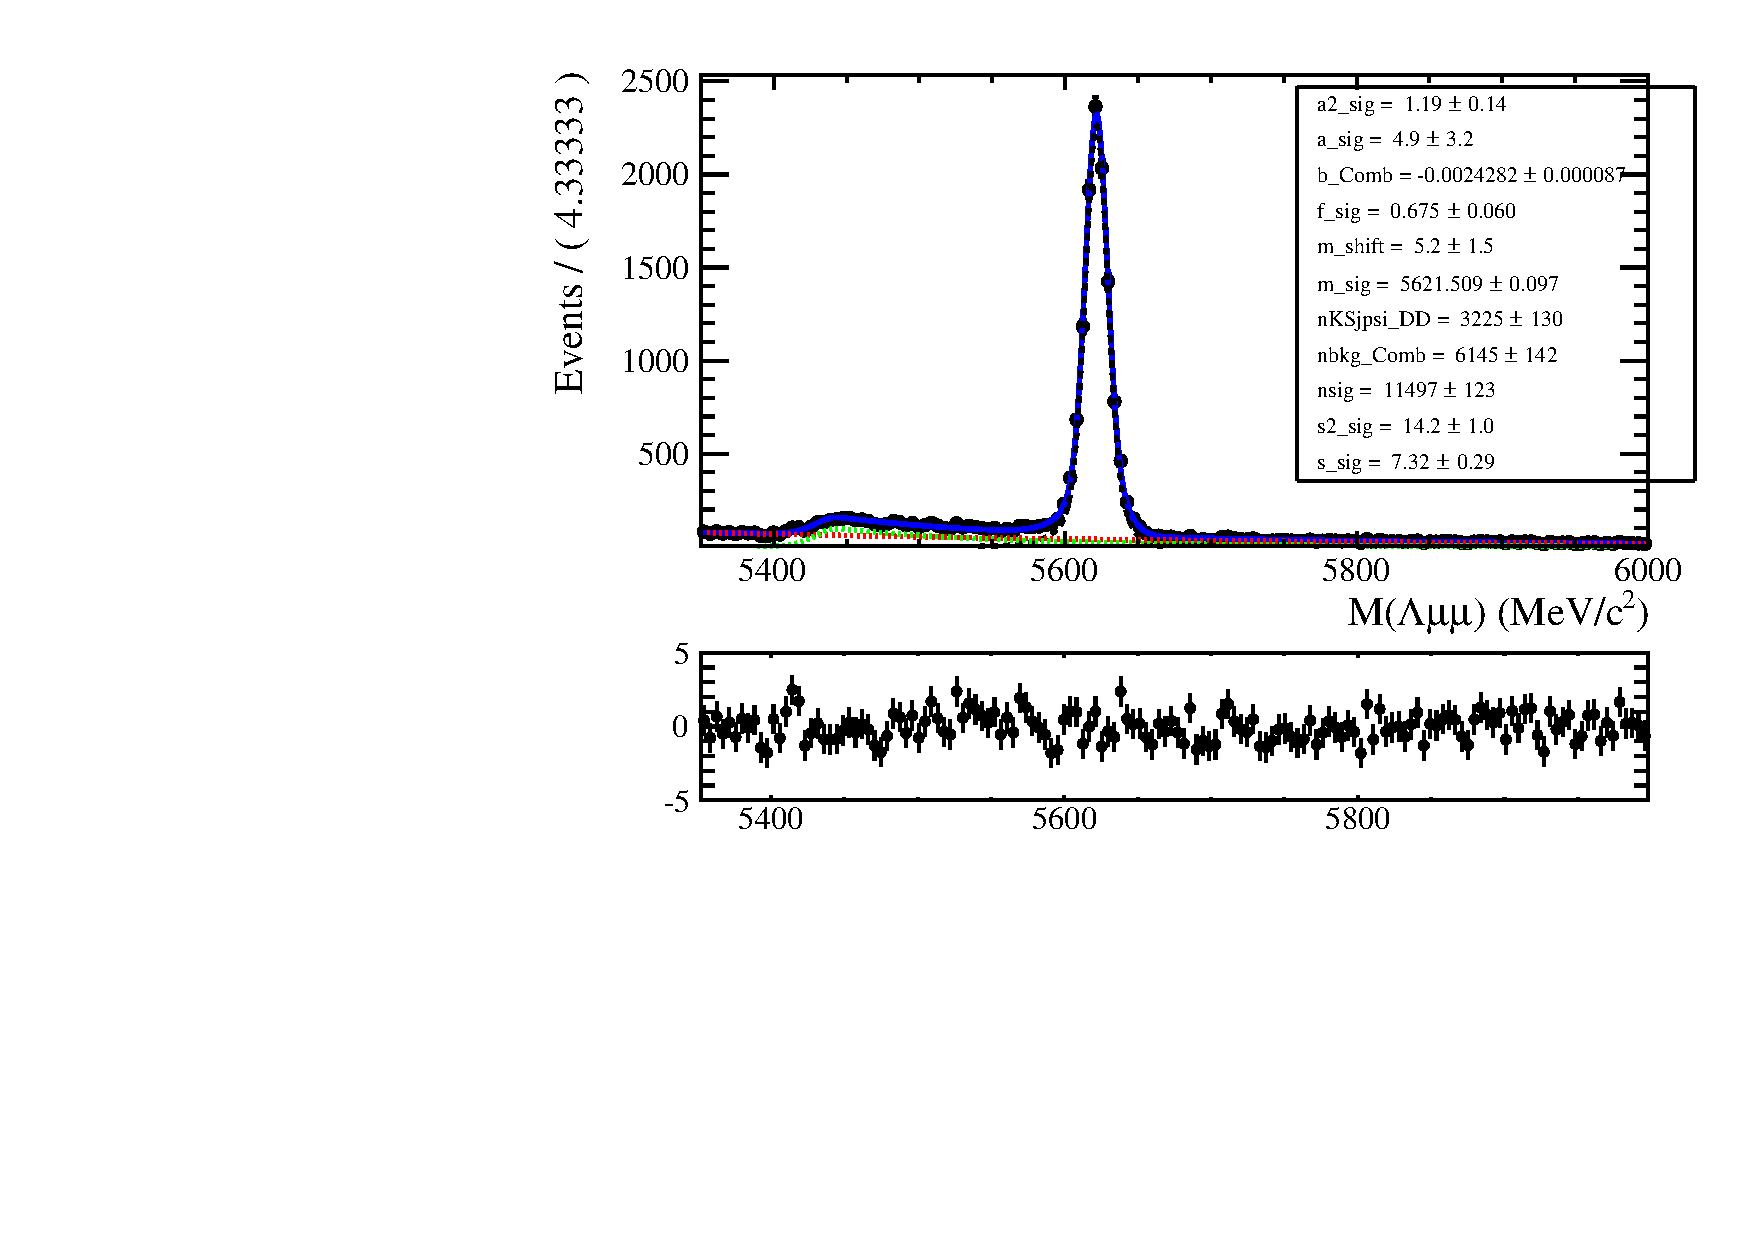
\includegraphics[width=0.45\textwidth]{Lmumu/figs/MassFits/Lb2JpsiL_DD_data_fitAndRes.pdf}
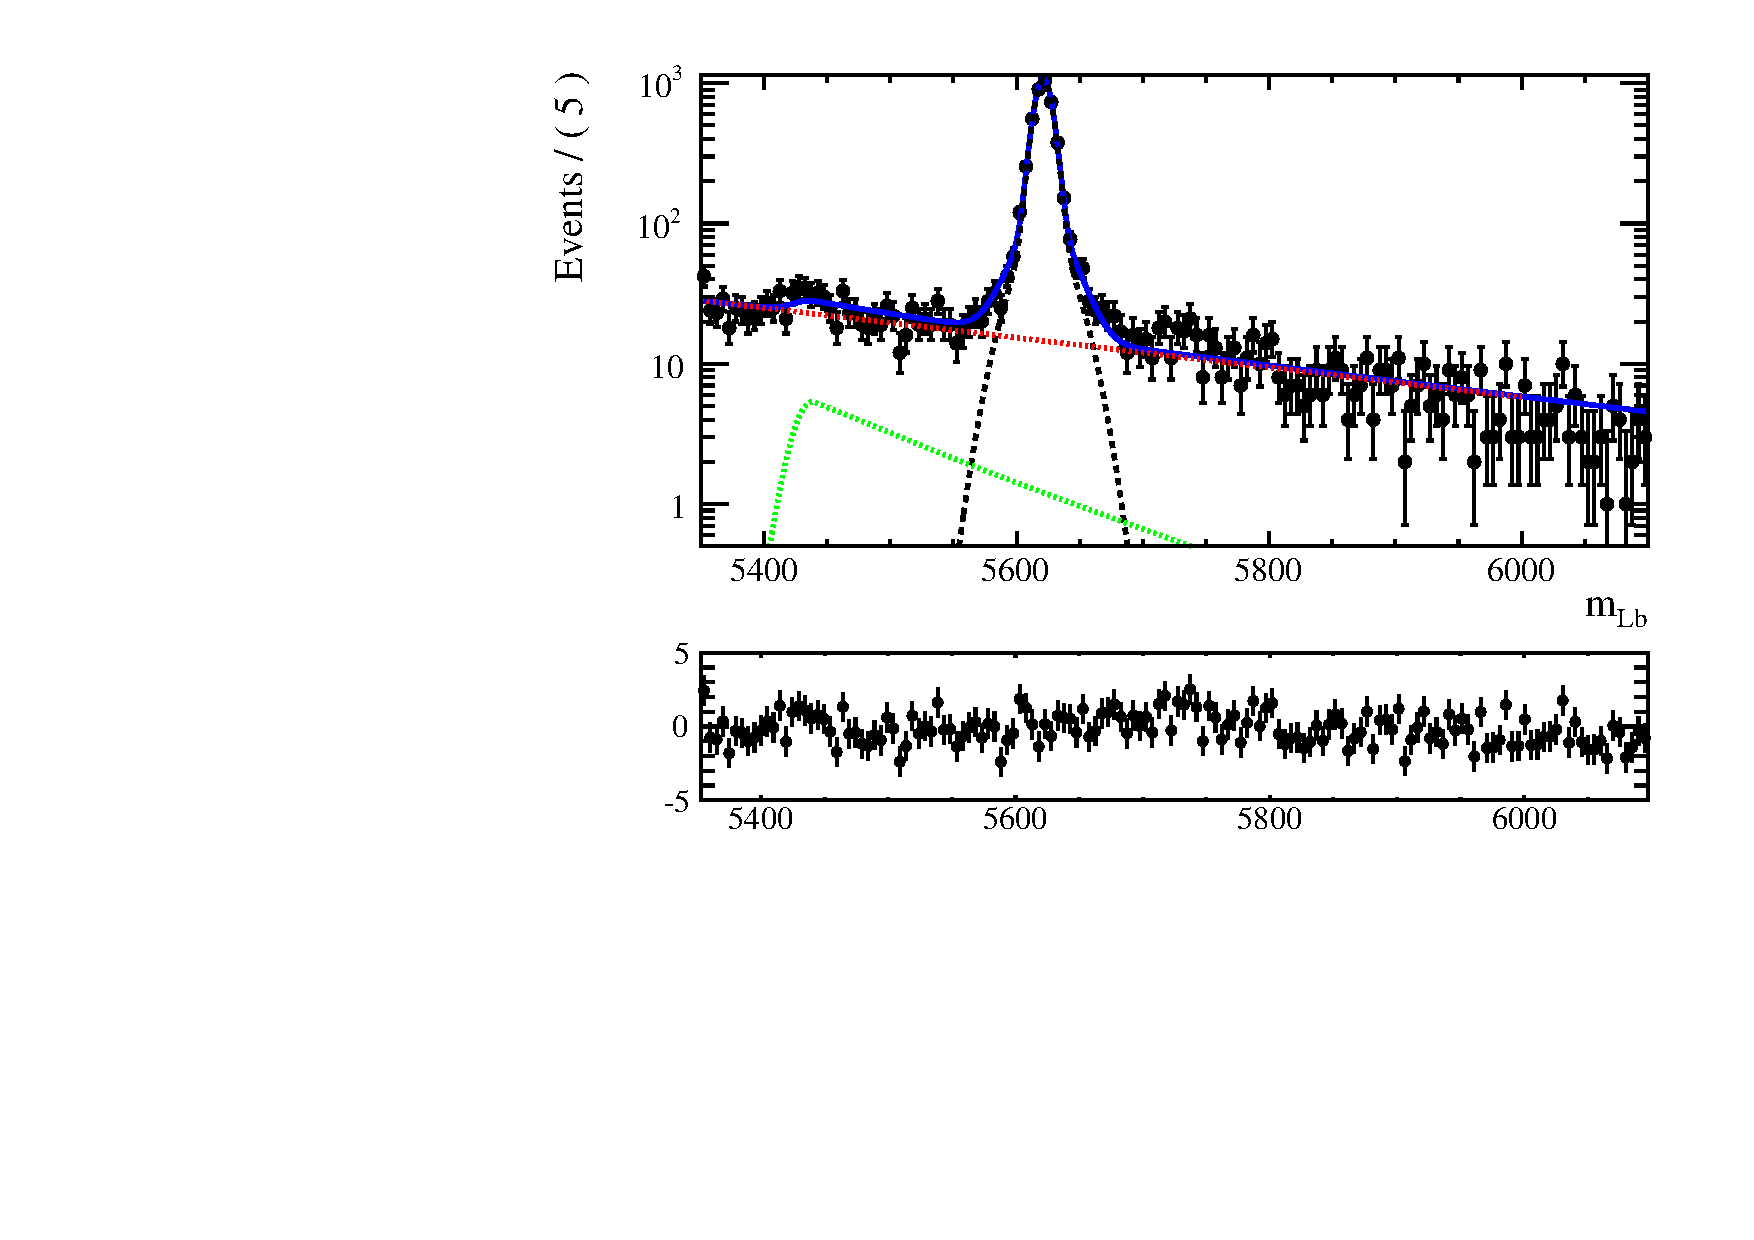
\includegraphics[width=0.45\textwidth]{Lmumu/figs/MassFits/Lb2JpsiL_LL_data_log_fitAndRes.pdf}
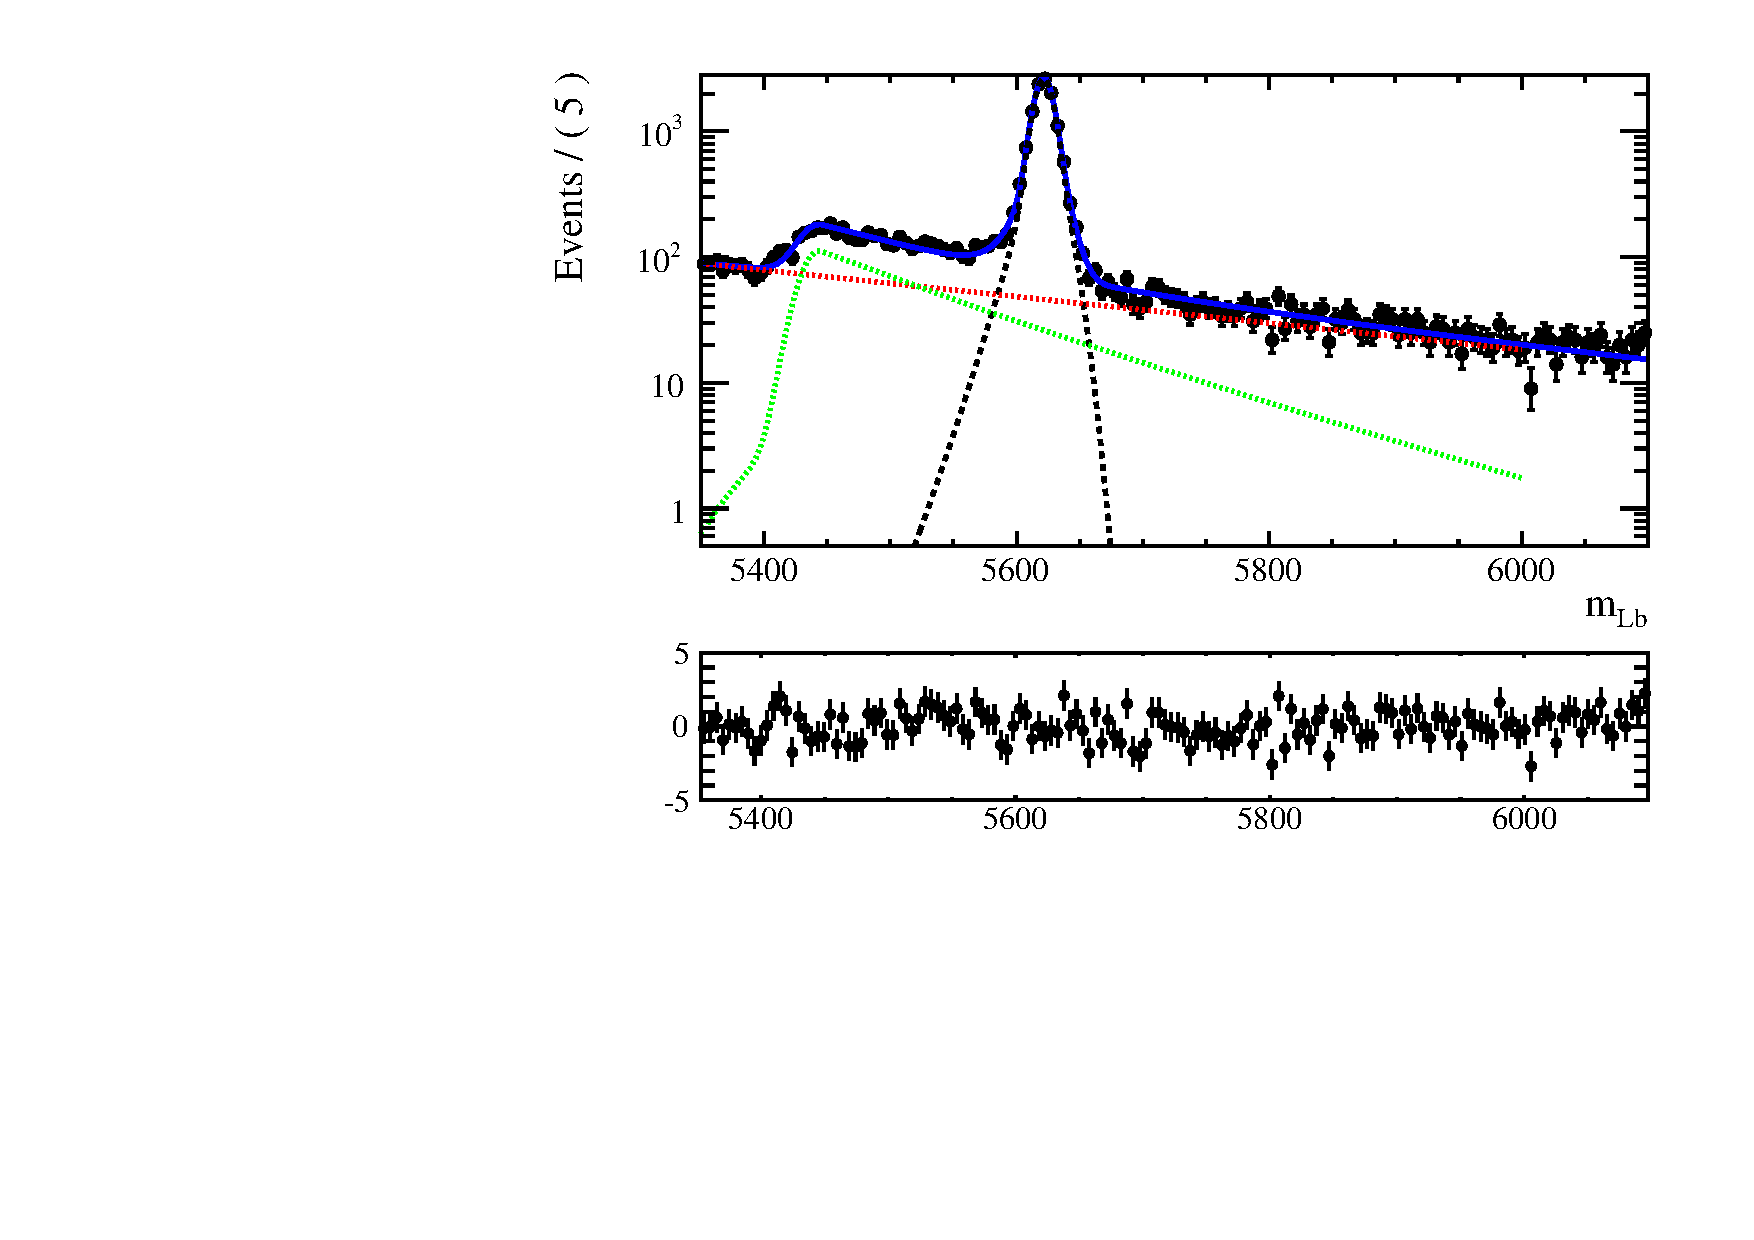
\includegraphics[width=0.45\textwidth]{Lmumu/figs/MassFits/Lb2JpsiL_DD_data_log_fitAndRes.pdf}
\caption{Invariant mass distribution of $\Lb\ra\jpsi\Lz$ and residuals of the fit for long-long (left) and 
down-down (right) events. Lower plots are the same as the upper ones but shown in linear scale.
The histogram shows data. On the plot are shown the total fit (blue line), the signal (black
dashed), the combinatorial background (red dashed) and the $\Bz\ra\KS\mumu$ background (green dashed).}
\label{fig:Lb_totalFit}
\end{figure}
%
In Fig.~\ref{fig:Lb_totalFit} are shown fitted invariant mass distributions for the normalisation channel,
selected with the high \qsq requirements and in Fig.~\ref{fig:Lb_totalFit_low} for low \qsq requirements.
%The $\chi^2$ value of the fit is $126$ for LL and $112$ for DD both with 140 degrees of freedom, which corresponds to probability of 80\% and 95\%.
Table~\ref{tab:Lb_rawYieldJpsi} reports measured yields of $\Lb\ra\jpsi\Lz$ candidates found using the low and high \qsq selections.
Values for the signal shape parameters are shown on Fig.~\ref{fig:Lb_totalFit}.
Results of the fit to the rare $\Lb\ra\Lz\mumu$ sample are shown in Fig.~\ref{fig:totalFitRare} for the integrated
$15 < \qsq < 20$ \gevgevcccc interval and in Fig.~\ref{fig:Lb_LmumuLowQ2} for the $1.1 < \qsq < 6.0$ \gevgevcccc one.
The exponential slopes, the scale factors multiplied to the widths and the number of combinatorial events
found from these fits are reported in Tab.~\ref{tab:Lb_rareParam}.
Fitted invariant mass distribution in all other considered \qsq intervals are in Fig.~\ref{fig:Lb_differentialFit2}
for downstream candidates and Fig.~\ref{fig:Lb_differentialFit2} for long candidates together with their significances.
The yields of rare events obtained from the fit are reported in Tab.~\ref{tab:Lb_rawYield}.
Most candidates are found in the downstream sample comprising $\sim 80\,\%$ of the total yield.
Notice that, since the fit is simultanous on DD and LL candidates, the yields in the two categories yields
are not parameters free to float independently in the fit but are correlated via the branching ratio.
The statistical significance of the observed signal yields is evaluated as $\sqrt{2\Delta\ln{\mathcal{L}}}$, where
$\Delta\ln{\mathcal{L}}$ is the change in the logarithm of the likelihood function when the signal component
is excluded from the fit, relative to the nominal fit in which it is present.

\begin{table}
\centering
\caption{Number of \decay{\Lb}{\jpsi\Lz} decays in the long and
  downstream categories found using the selection for low- and
  high-\qsq regions. Uncertainties shown are statistical only.}
\begin{tabular}{lcc}
Selection & $N_{\rm S}$ (long) & $N_{\rm S}$ (downstream)\\ \hline
high-\qsq	& $4313 \pm 70$	 	&  $11\,497 \pm 123$ \\
low-\qsq	& $3363 \pm 59$ 	&  $\phantom{0}\,7225 \pm 89\phantom{0}$  \\
 \hline
\end{tabular}
\label{tab:Lb_rawYieldJpsi}
\end{table}



\begin{table}
\centering
\caption{Signal decay yields ($N_\mathrm{S}$) obtained from the
  mass fit to \decay{\Lb}{\Lz\mumu} candidates in each \qsq interval
  together with their statistical significances. 
  The $8-11$ and $12.5-15$ \gevgevcccc ~\qsq intervals are excluded
  from the study as they are dominated by decays via charmonium resonances.}
\begin{tabular}{lcccc} \hline\hline
 \qsq interval [\gevgevcccc] & DD & LL & Tot. yield & Significance \\ \hline
0.1 -- 2.0    &  $6.9 \pm 2.2$  &  $9.1 \pm 3.0$	 &  $16.0\pm5.3$            			 &  4.4 \\
2.0 -- 4.0    &  $1.8 \pm 1.7$  &  $3.0 \pm 2.8$ 	 &  $\phantom{0}4.8\pm4.7$  			 &  1.2 \\
4.0 -- 6.0    &  $0.4 \pm 0.9$  &  $0.6 \pm 1.4$	 &  $\phantom{0}0.9\pm2.3$  			 &  0.5 \\
6.0 -- 8.0    &  $4.3 \pm 2.0$   &  $7.2 \pm 3.3$	 &  $11.4\pm5.3$            			 &  2.7 \\
11.0 -- 12.5  &	 $14.6 \pm 2.9$  &  $42.8 \pm 8.5$   &  $\phantom{.0}60\pm12\phantom{.}$    &  6.5 \\
15.0 -- 16.0  &  $13.5 \pm 2.2$  &  $43.5 \pm 7.2$   &  $57\pm9$                			 &  8.7 \\
16.0 -- 18.0  &  $28.6 \pm 3.3$  &  $88.8 \pm 10.1$	 &  $118\pm13$              			 &  13  \\
18.0 -- 20.0  &  $22.4 \pm 2.6$  &  $78.0 \pm 8.9$	 &  $\phantom{.}100\pm11\phantom{.}$    &  14  \\
\hline
1.1 -- 6.0    &  $3.6 \pm 2.4$  &  $5.7 \pm 3.8$	 &  $\phantom{0}9.4\pm6.3$  			&  1.7 \\
15.0 -- 20.0  &  $64.6 \pm 4.7$  &  $209.6 \pm 15.3$ &  $276\pm20$              			&  21  \\
\end{tabular}
\label{tab:Lb_rawYield}
\end{table}

\begin{figure}
\centering
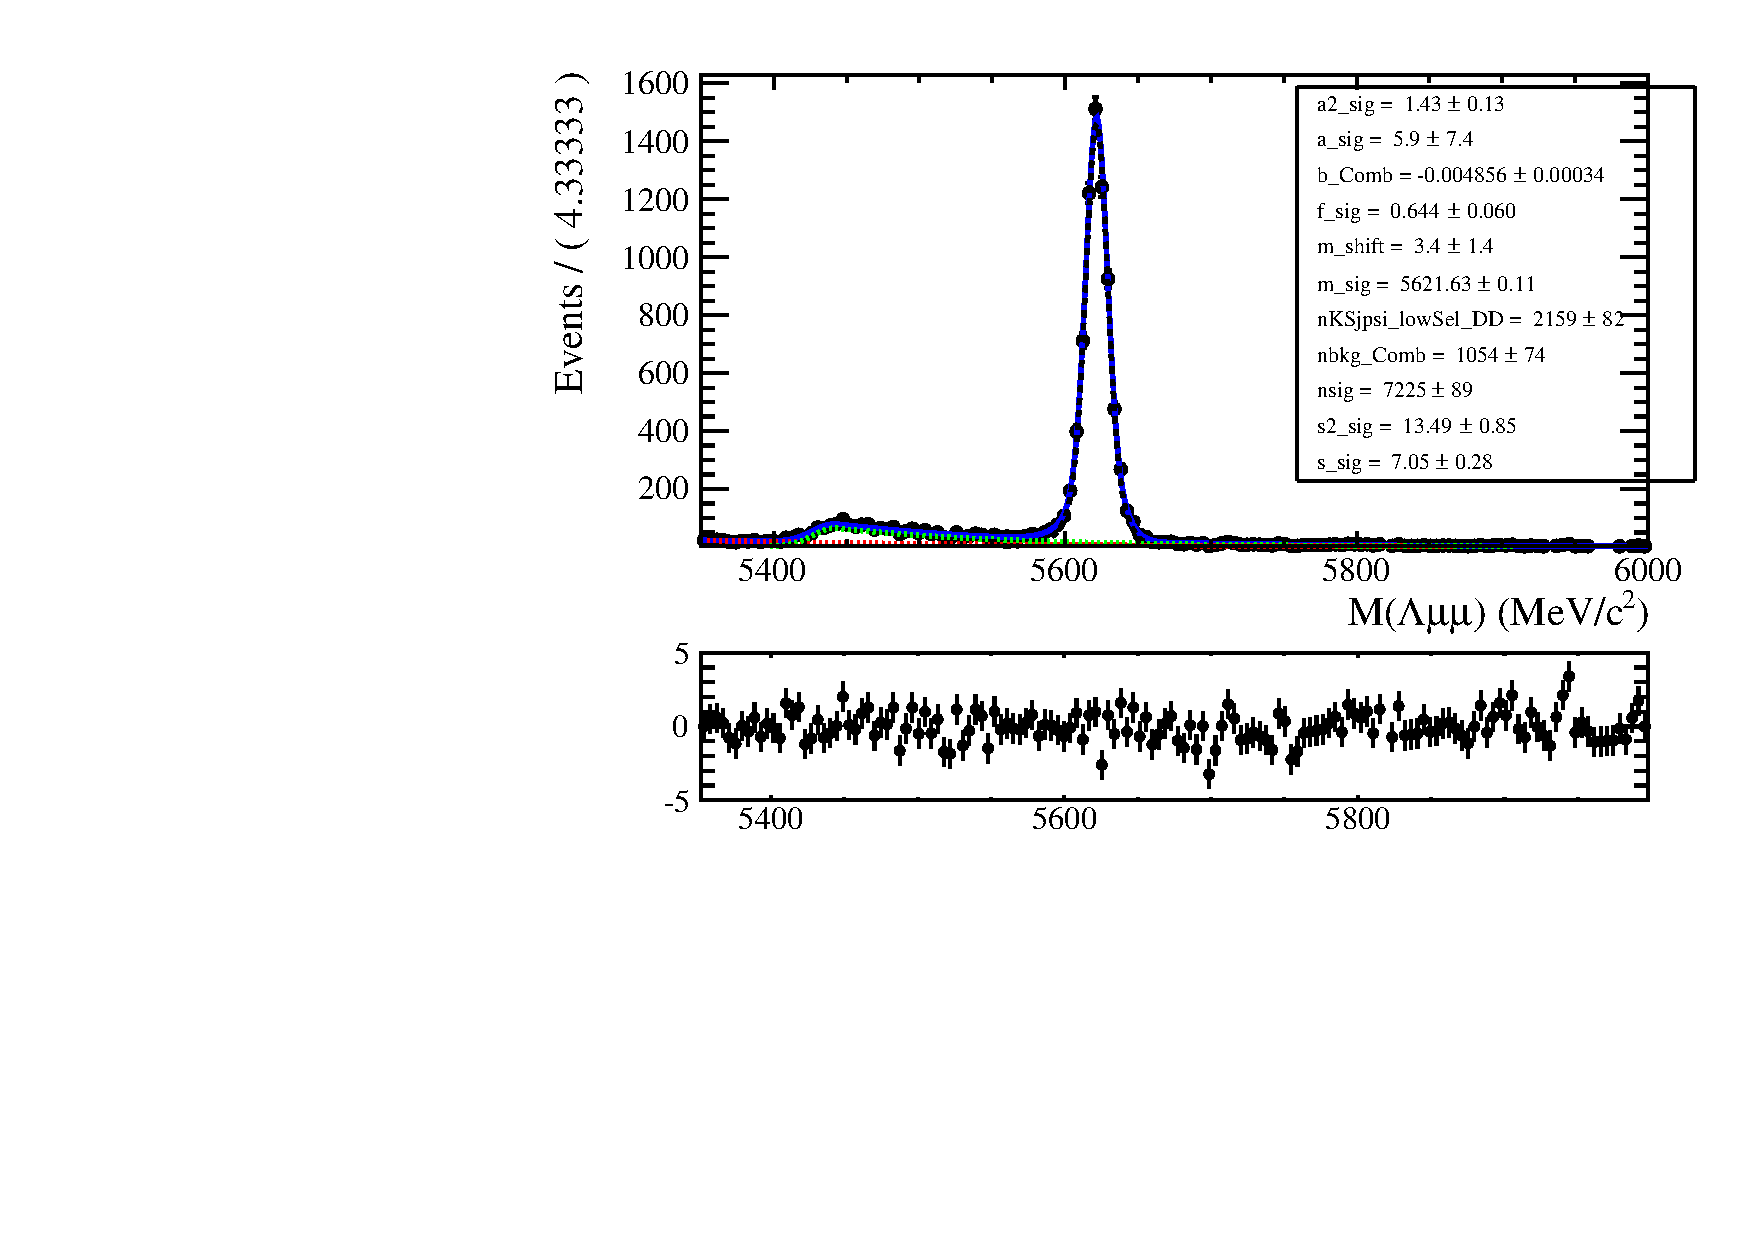
\includegraphics[width=0.45\textwidth]{Lmumu/figs/MassFits/Lb2JpsiL_lowSel_DD_data_fitAndRes.pdf}
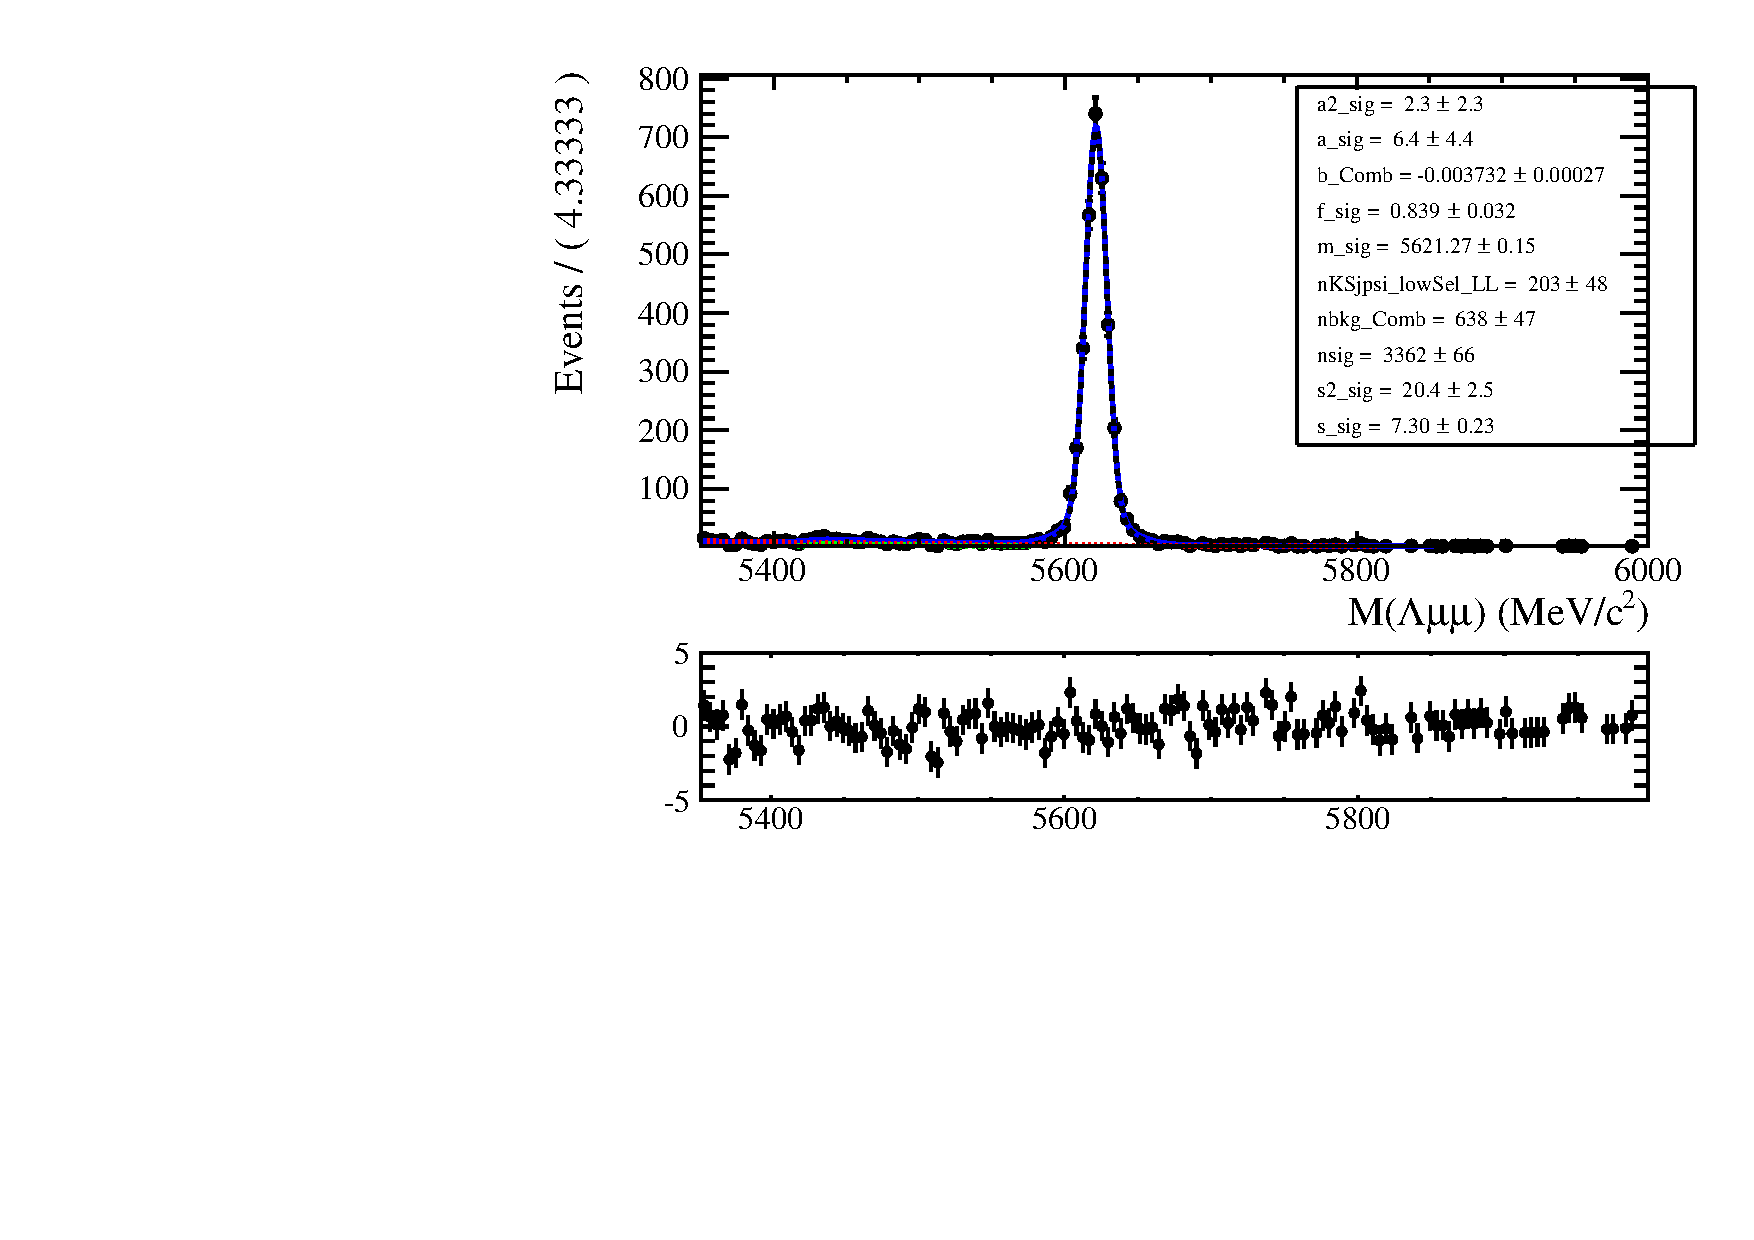
\includegraphics[width=0.45\textwidth]{Lmumu/figs/MassFits/Lb2JpsiL_lowSel_LL_data_fitAndRes.pdf}
\caption{Invariant mass distribution of $\Lb\ra\Lz\jpsi$ with fit and residuals for DD events (left) and LL events (right).
The histogram shows real data selected with low \qsq selection. The blue line is the total fit function.}
\label{fig:Lb_totalFit_low}
\end{figure}
%
\begin{figure}
\centering
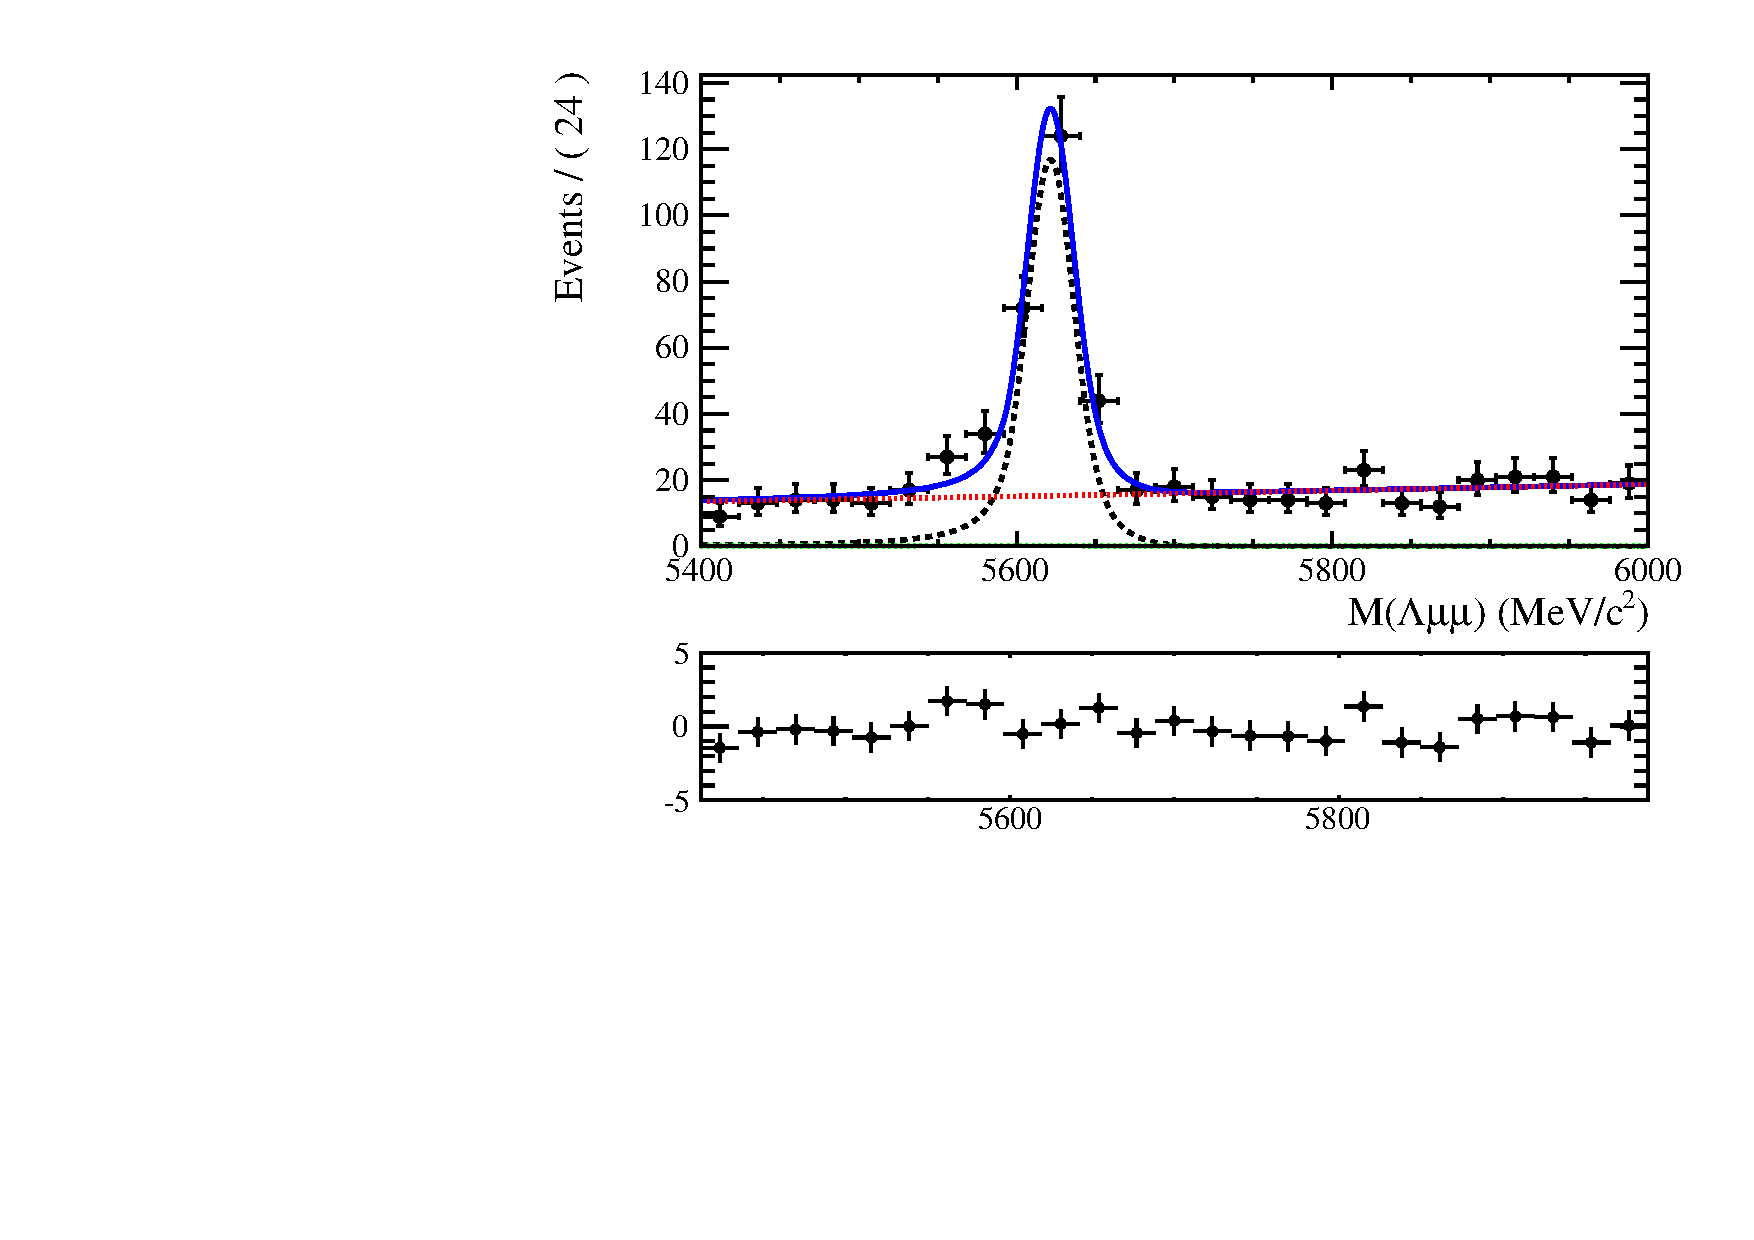
\includegraphics[width=0.45\textwidth]{Lmumu/figs/MassFits/Lb2Lmumu_DD_highQ2_fitAndRes.pdf}
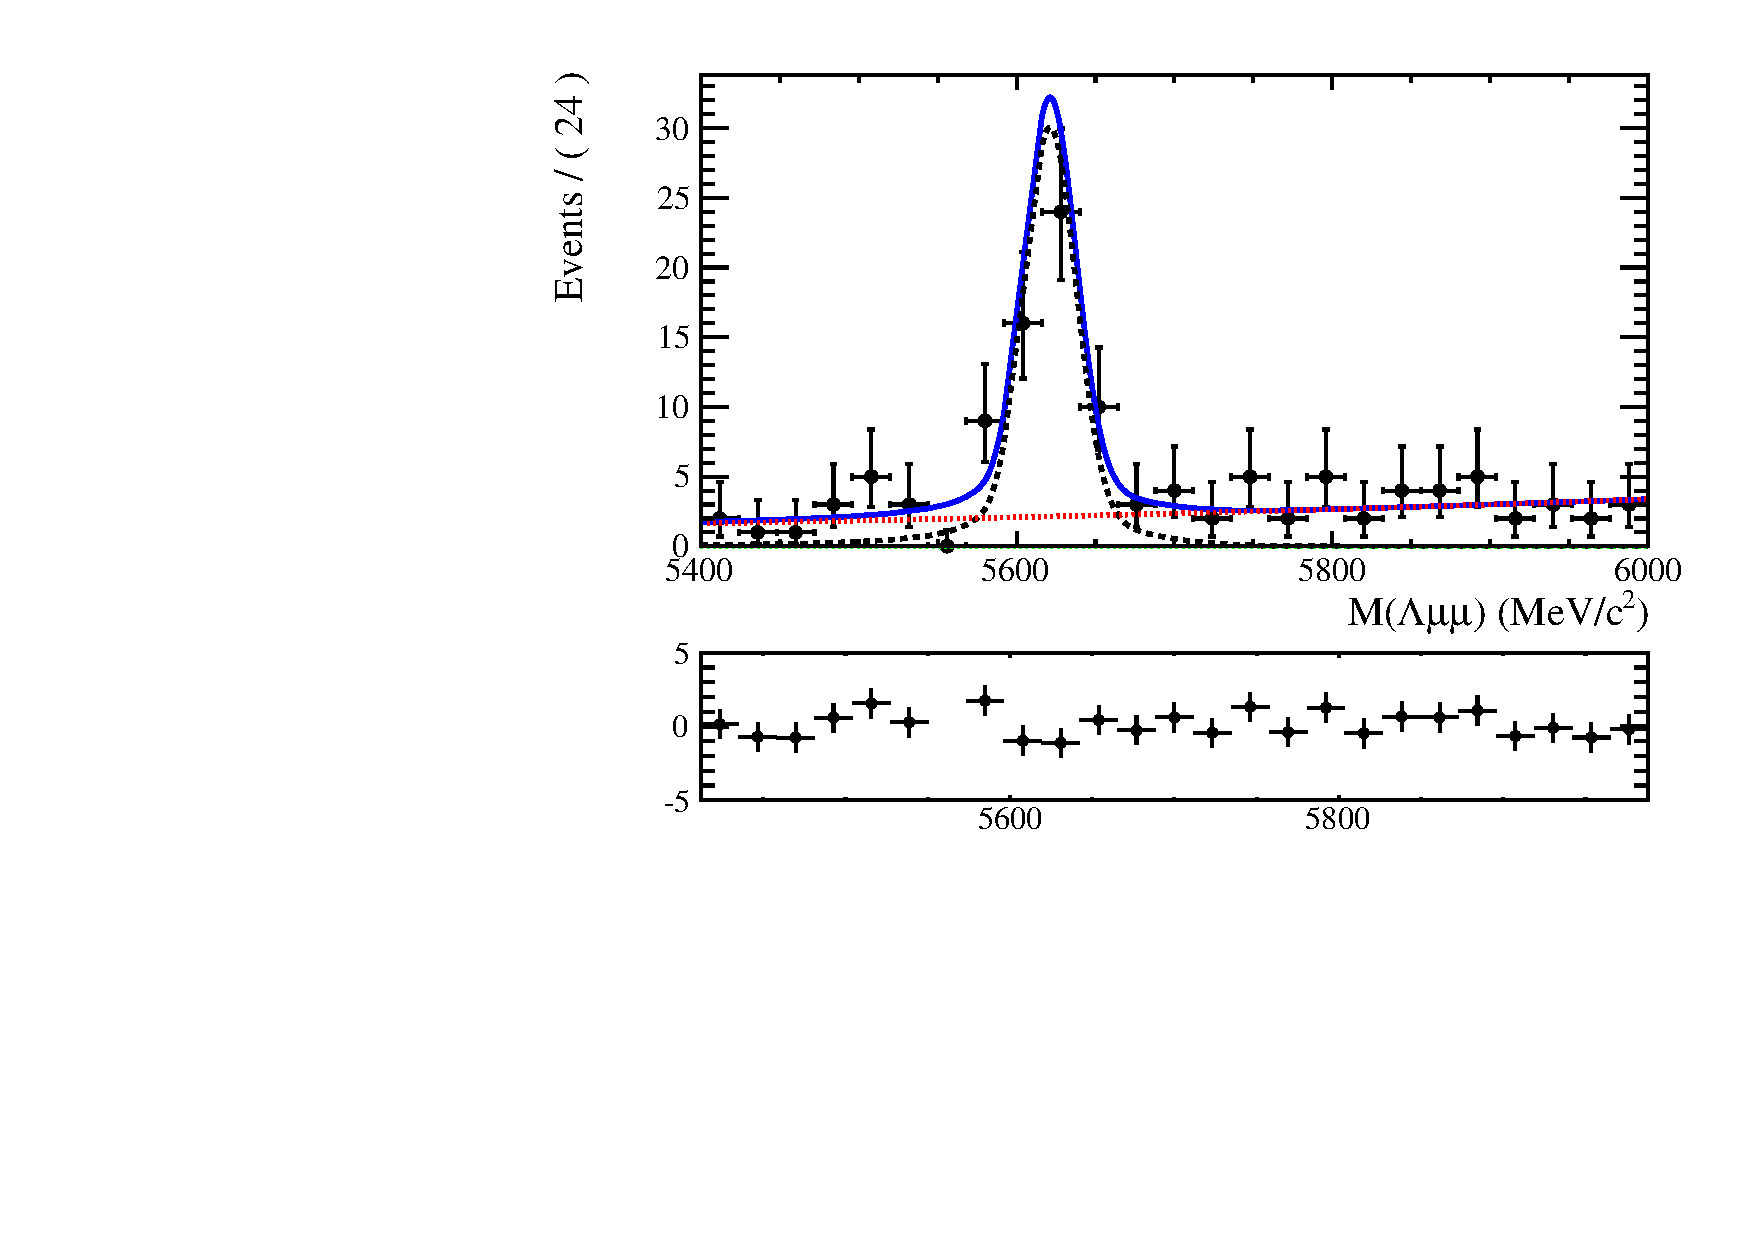
\includegraphics[width=0.45\textwidth]{Lmumu/figs/MassFits/Lb2Lmumu_LL_highQ2_fitAndRes.pdf}
\caption{Invariant mass distribution of rare $\Lb\ra\Lz\mumu$ for downstream (left) and long (right) condidates
in the integrated 15--20 \gevgevcccc ~\qsq interval. The points show data, the blue line
the total fit function and the dashed red line represents combinatorial background.}
\label{fig:Lb_totalFitRare}
\end{figure}
%
%
\begin{figure}
\centering
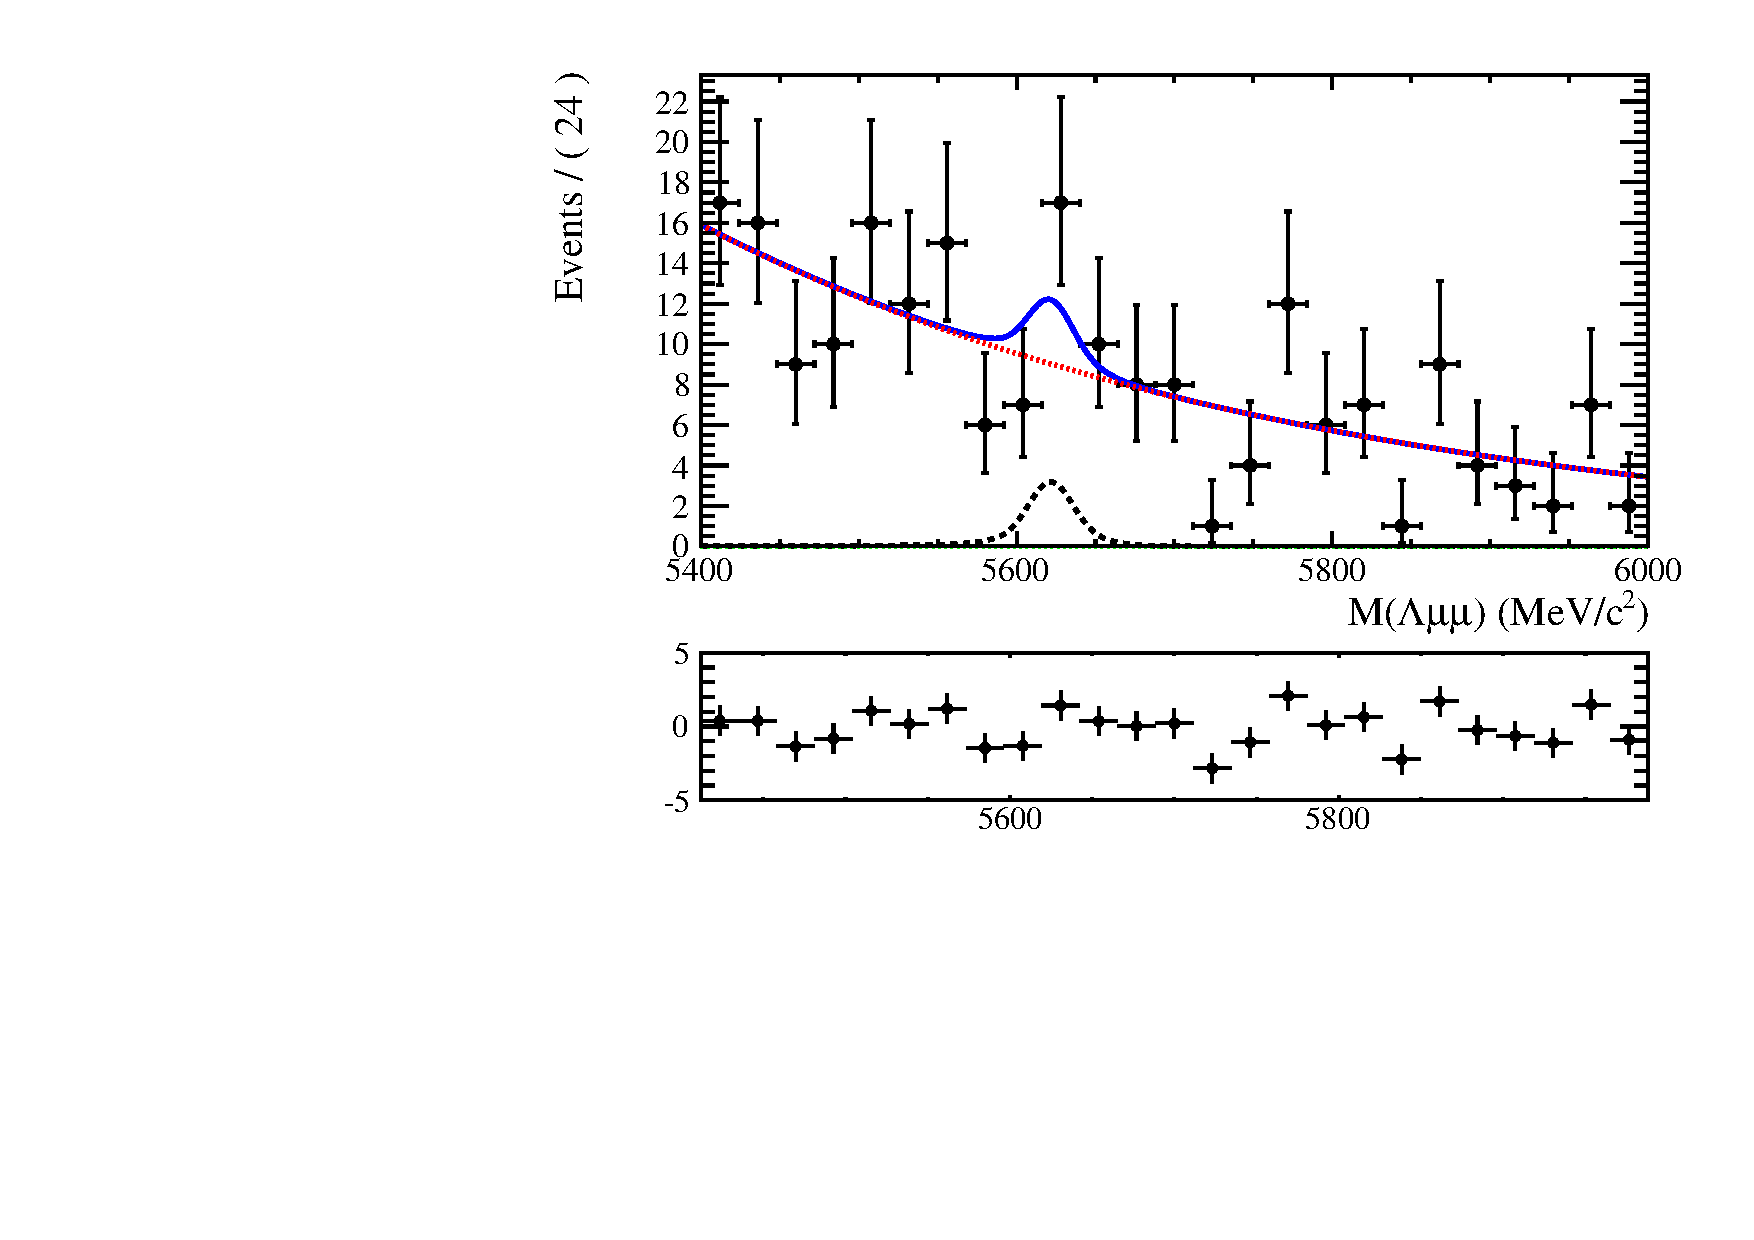
\includegraphics[width=0.45\textwidth]{Lmumu/figs/MassFits/Lb2Lmumu_DD_lowQ2_fitAndRes.pdf}
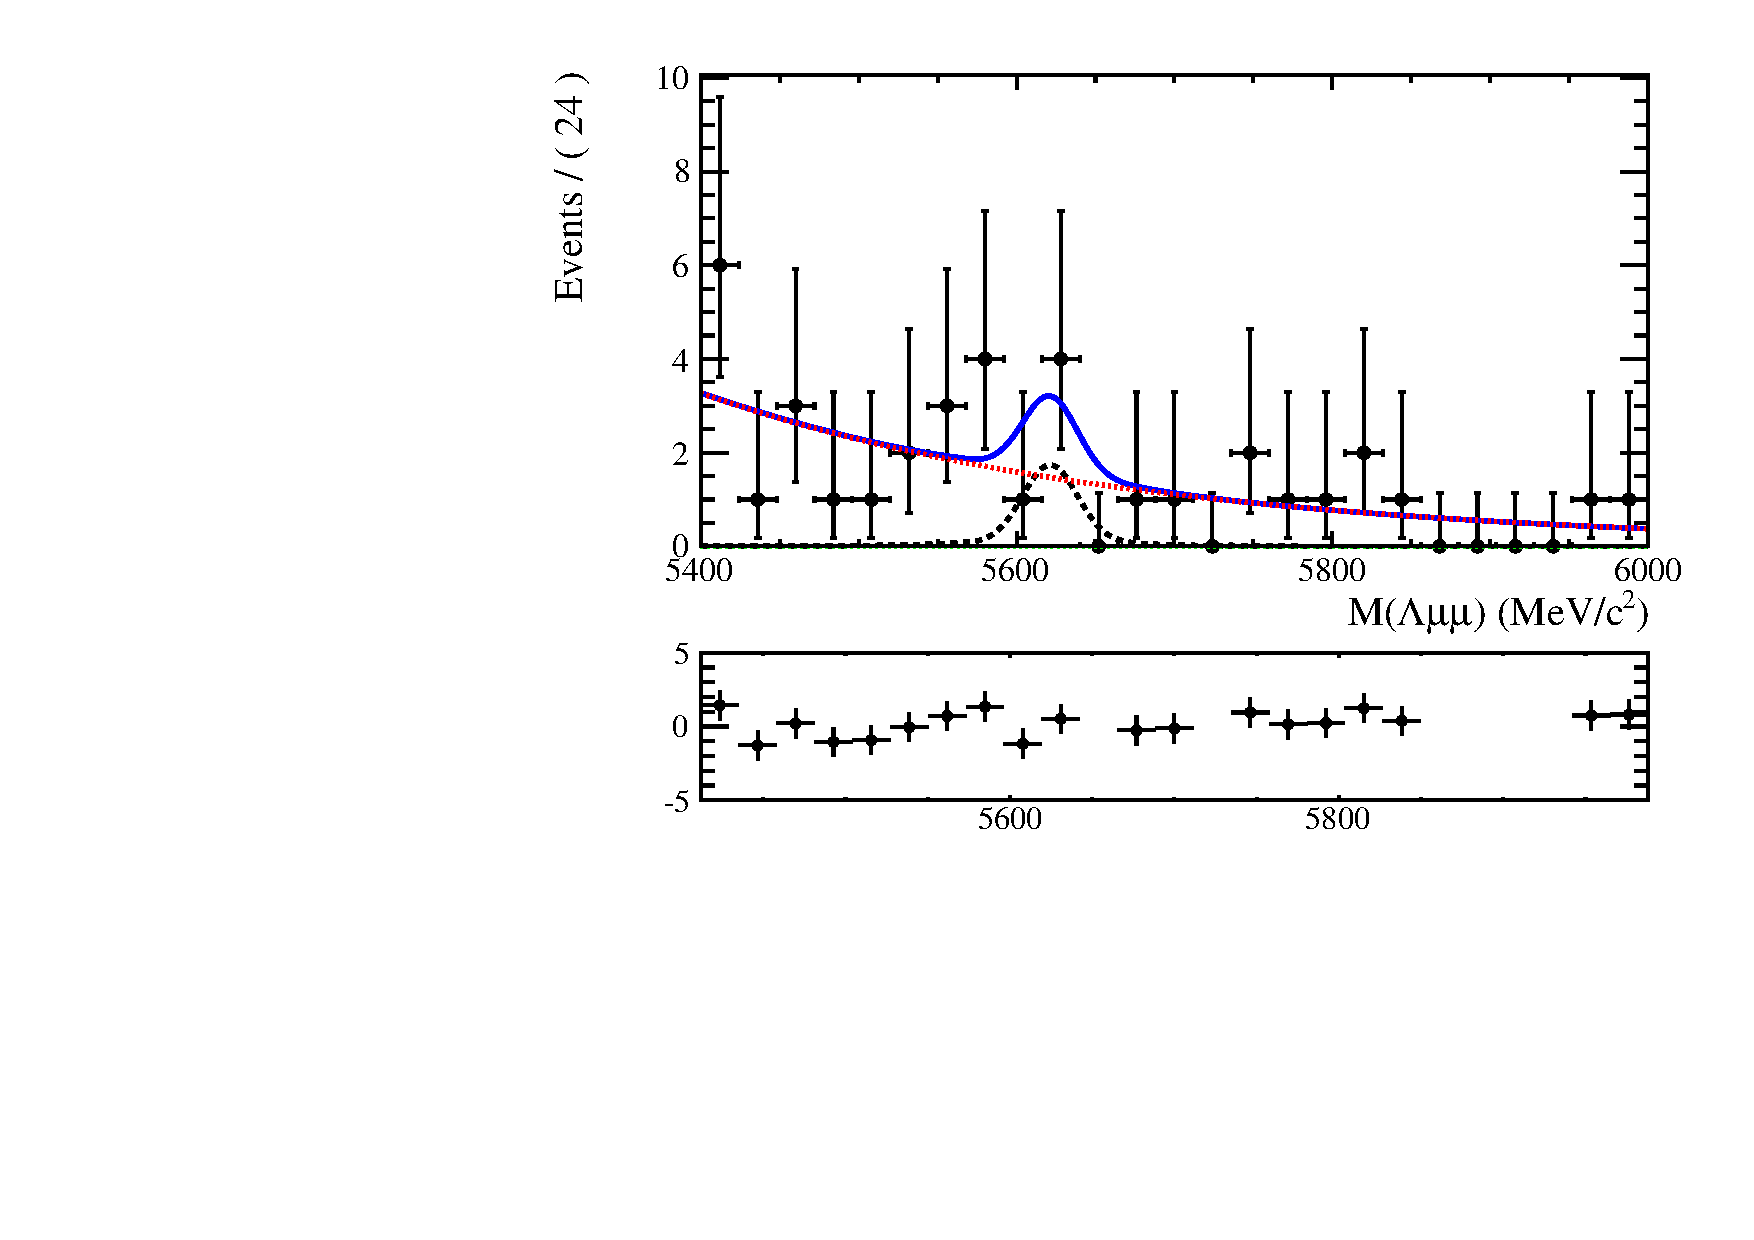
\includegraphics[width=0.45\textwidth]{Lmumu/figs/MassFits/Lb2Lmumu_LL_lowQ2_fitAndRes.pdf}
\caption{Invariant mass distribution of $\Lb\ra\Lz\mumu$ candidates in the integrated 0.1--6.0 
\gevgevcccc ~\qsq interval for downstream (left) and long (right) candidates. The points show data, the blue line
the total fit function and the dashed red line represents combinatorial background.}
\label{fig:Lb_LmumuLowQ2}
\end{figure}
%
\begin{figure}
\centering
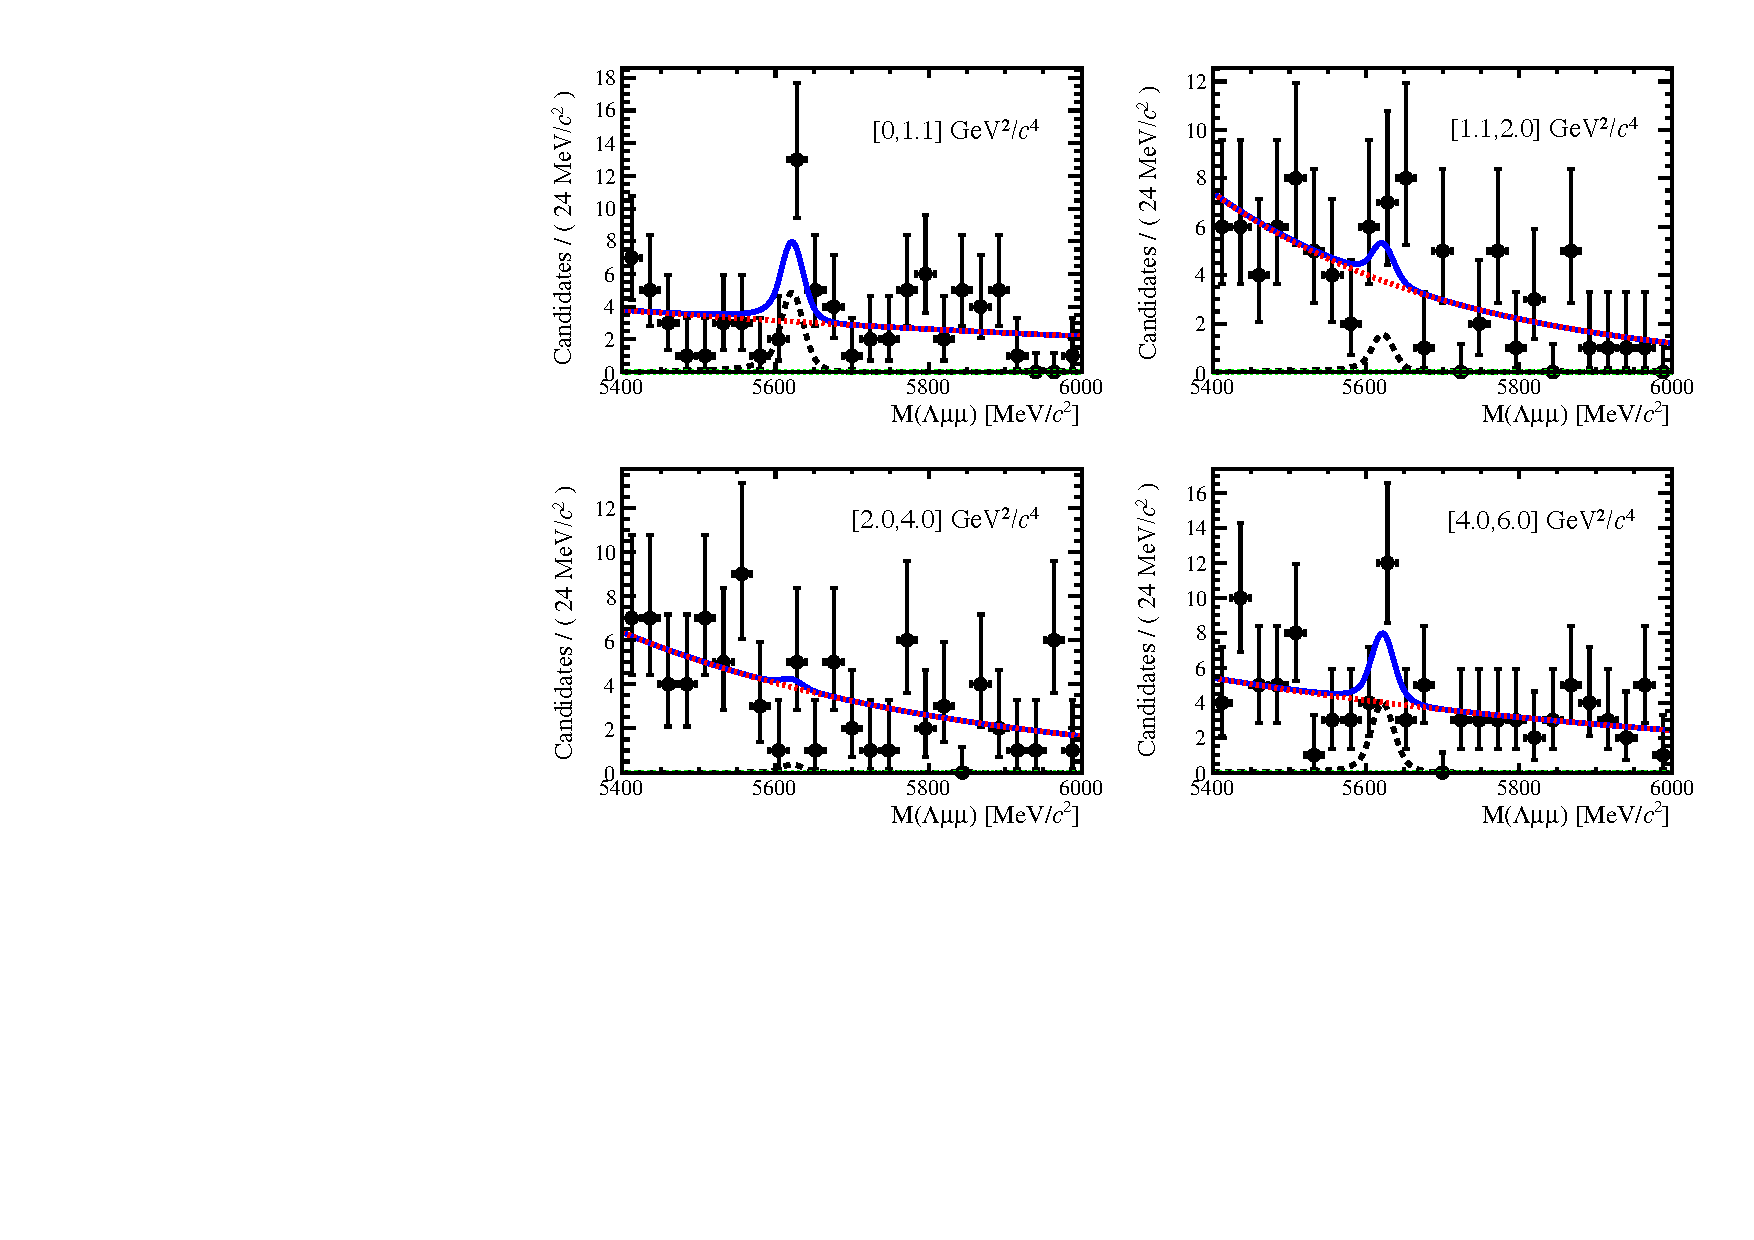
\includegraphics[width=0.8\textwidth]{Lmumu/figs/MassFits/q2_fits_DD_plot2.pdf}
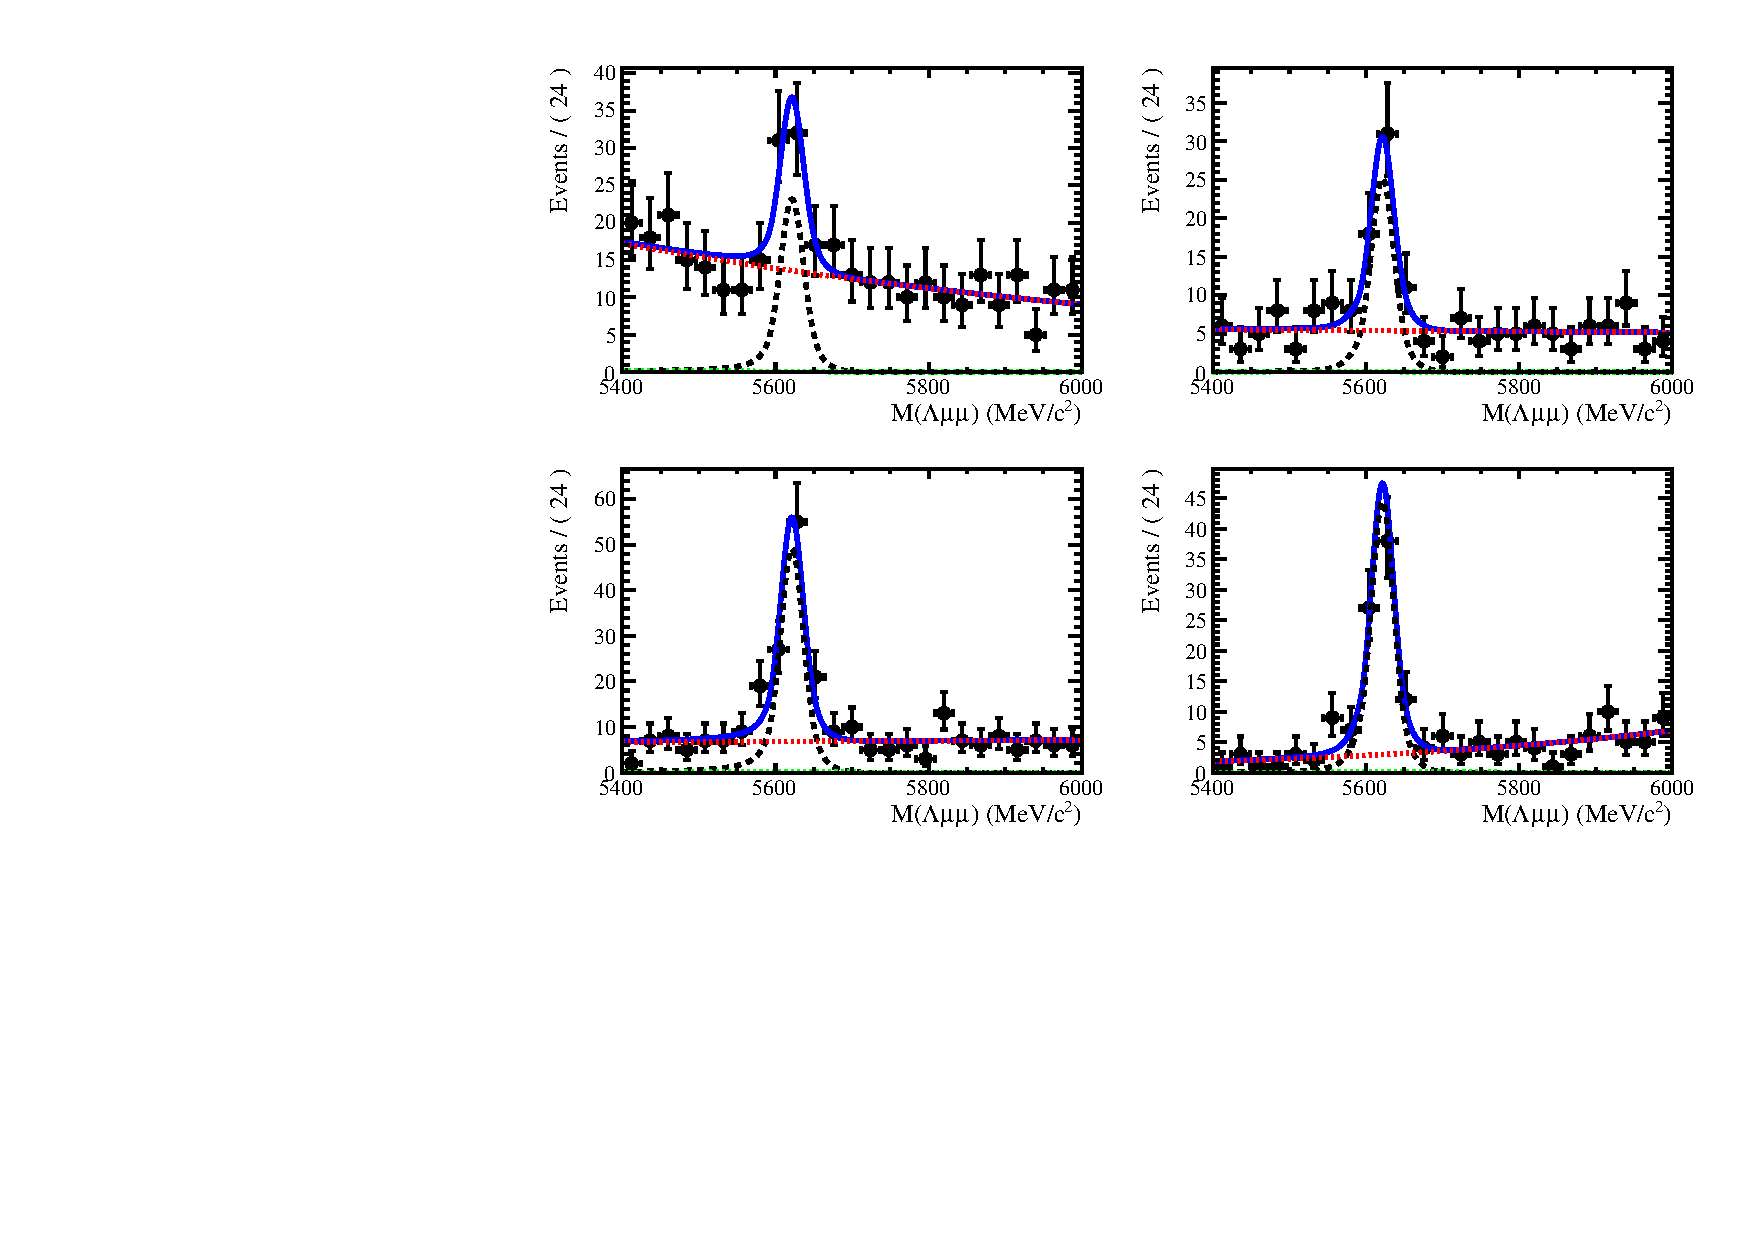
\includegraphics[width=0.8\textwidth]{Lmumu/figs/MassFits/q2_fits_DD_plot1.pdf}
\caption{Invariant mass distributions of rare $\Lb\ra\Lz\mumu$ candidates in the considered \qsq bins
 %[0.1,2], [2,4], [4,6], [6,8], [11,12.5], [15,16], [16,18], [18,20]
 for downstream candidates. }
\label{fig:Lb_differentialFit}
\end{figure}

\begin{figure}
\centering
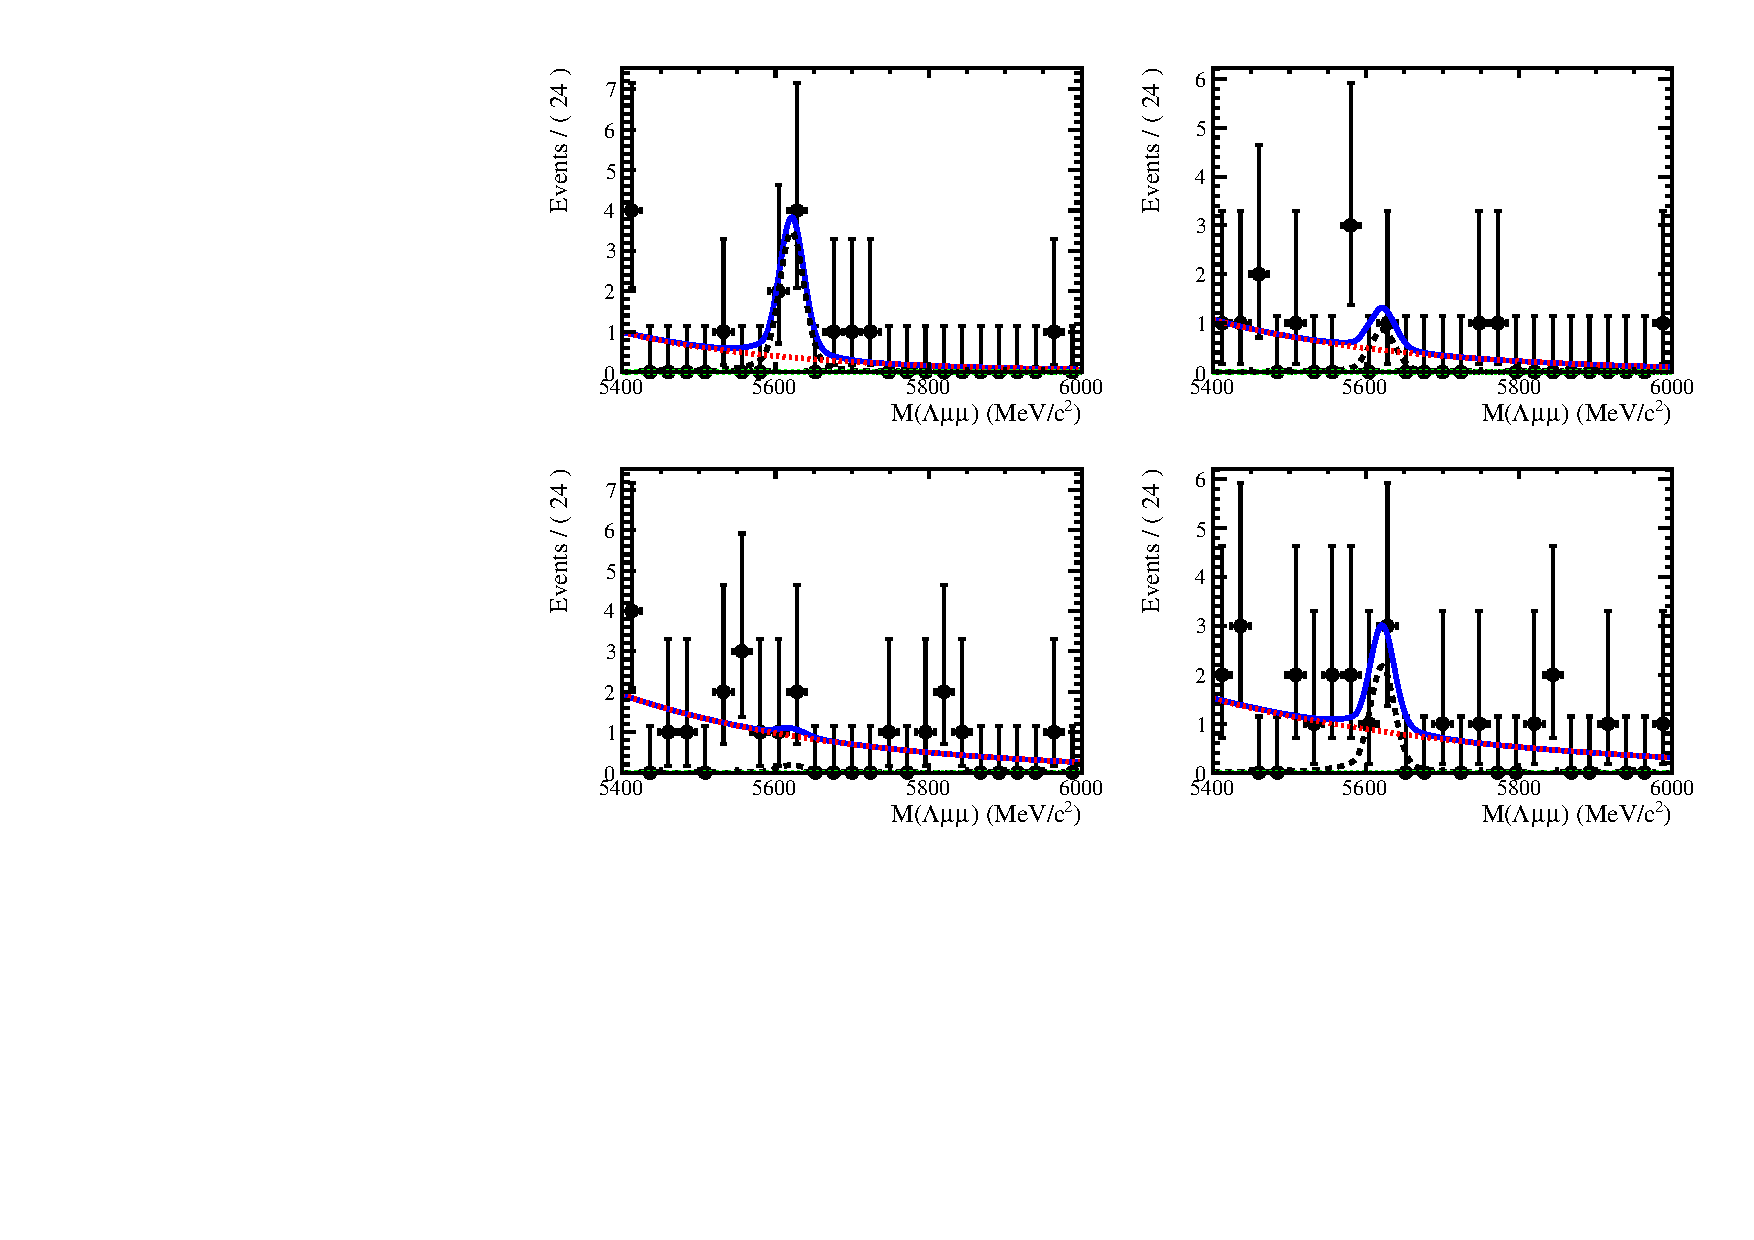
\includegraphics[width=0.8\textwidth]{Lmumu/figs/MassFits/q2_fits_LL_plot2.pdf}
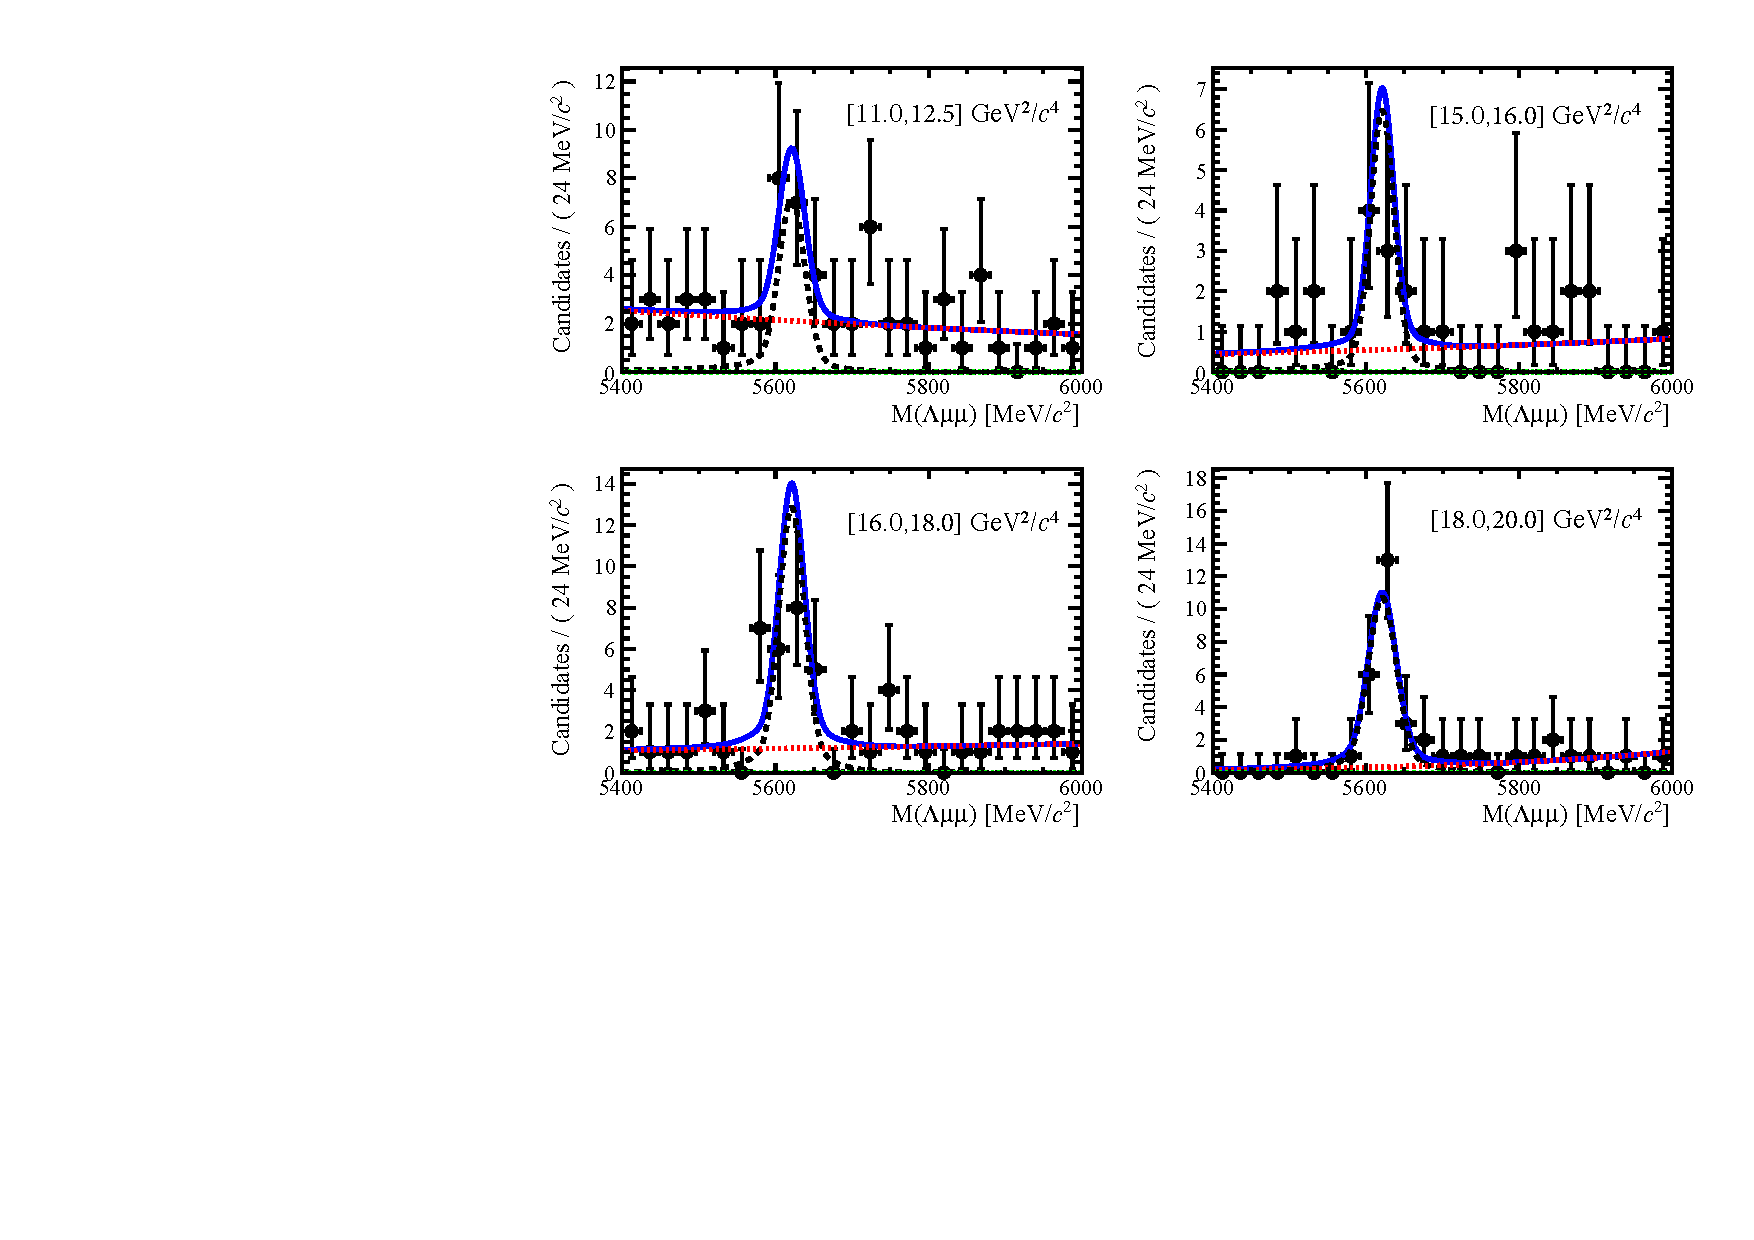
\includegraphics[width=0.8\textwidth]{Lmumu/figs/MassFits/q2_fits_LL_plot1.pdf}
\caption{Invariant mass distributions of rare $\Lb\ra\Lz\mumu$ candidates in the considered \qsq bins
 %[0.1,2], [2,4], [4,6], [6,8], [11,12.5], [15,16], [16,18], [18,20]
 for long candidates. }
\label{fig:Lb_differentialFitLL}
\end{figure}



%\begin{table}
%\centering
%\caption{Values of exponential slope, $b$, and scale factors, $c$ found from the fit
%to the resonant data sample and fixed from the fit to the rare data sample.}
%\begin{tabular}{|c|c|c|}
%\hline
%Parameter  			 & Downstream & Long	\\ 
%\hline
%\multicolumn{3}{|c|}{ 15.0--20.0 \gevgevcccc}  \\
%\hline

%$b$ 				& $0.0006 \pm 0.0003$		 		& 	$0.0012 \pm 0.0008$        \\
%$c$ 				& $1.9027 \pm 0.0001$ 				&	$2.2910 \pm 0.0001$        \\
%%$N_{exp}$ 			& $393^{+23}_{-22}$	&	 $64^{+9}_{-8}$       \\

%\hline
%\multicolumn{3}{|c|}{ 1.1--6.0 \gevgevcccc}  \\

%\hline
%$b$ 				& $-0.0026 \pm 0.0004$				&	$-0.0036 \pm 0.0011$	 \\
%$c$ 				& $1.9208 \pm 0.0001$				&	$2.3504 \pm 0.0001$        \\
%%$N_{exp}$ 			& $203^{+15}_{-14}$	&	$34^{+7}_{-6}$       \\
%\hline

%\end{tabular}
%\label{tab:Lb_rareParam}
%\end{table}




\clearpage

